\newpage

\section{流水线ADC工作原理}
\subsection{数据转换的基本思路}
\begin{figure}[ht]
    \centering
    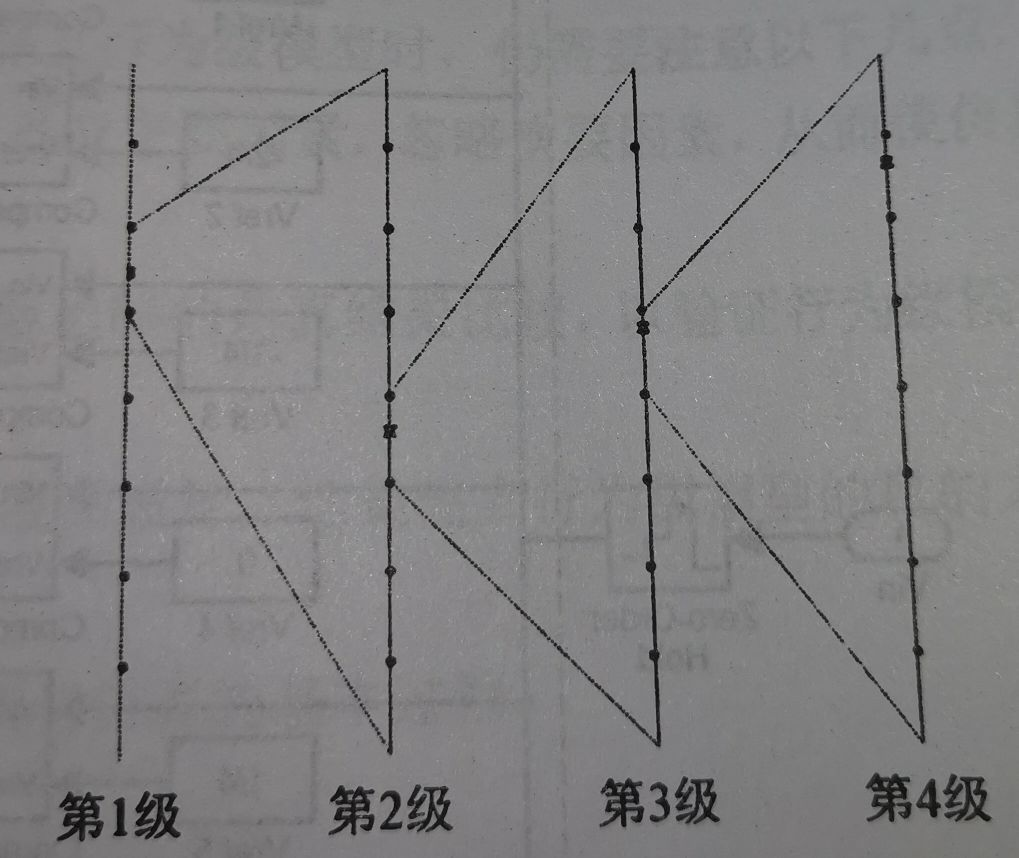
\includegraphics[width=8cm]{Pipeline_basic}
    \caption{\label{fig:pip-basic}流水线ADC的基本思路}
\end{figure}
如图2.1,以12bits的流水线ADC为例,利用4个三位子ADC的级联,使它们并行工作。
第一级ADC将输入信号量化到3位精度,将对应位置的精度再放大到满幅,第二级再将
输入信号量化3位,此时输出精度已经达到6位,一直到第四级ADC时,输出精度可以达到12位。

\subsection{流水线ADC的结构}
流水线ADC由多个结构相似功能相近的子转换电路组成,如图2.2。输入信号先经过采样保持电路,使电路输出
电压在每一个时钟信号之间都保持不变,不断跟踪输入信号的变化。后面的级联结构将输出精度分配到每一级上,
每个子转换电路输出一个转换结果。由于各级串行,对输入信号的转换逐级延迟,因此,子转换电路
的输出都接入一个延迟对准和数字校准电路中,在时序上对齐,并进行冗余位矫正。
\begin{figure}[ht]
    \centering
    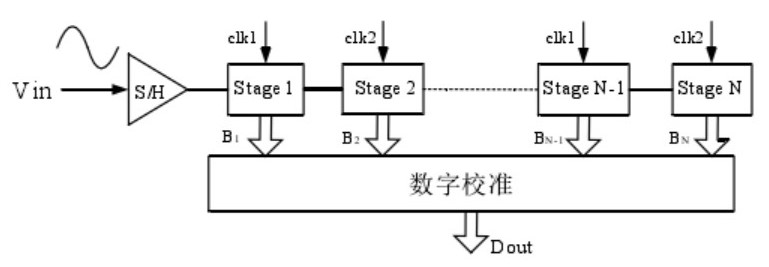
\includegraphics[width=8cm]{Pipeline_tradition}
    \caption{\label{fig:pip-tradition}流水线ADC的基本架构}
\end{figure}
\par 每一级子转换器电路由一个用于输出该级量化结果的sub-ADC和放大余量的MDAC构成。MDAC集成了
减法与放大功能,先将本级的输入与sub-ADC的输出做减法,再将余量放大$ 2^{k-1} $倍之后,输出到下一级。
直到最后一级无需继续进行余量放大,因此一般采用一个位数较高的Flash ADC。
\begin{figure}[ht]
    \centering
    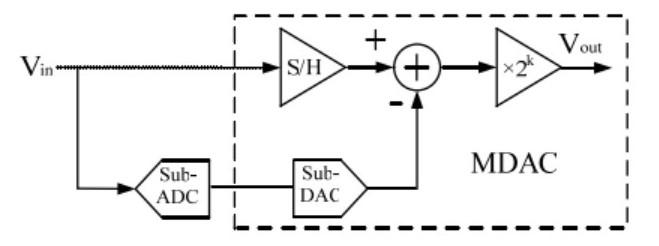
\includegraphics[width=8cm]{sub-Structure}
    \caption{\label{fig:sub-Structure}子转换级电路结构图}
\end{figure}
\subsubsection{sub-ADC电路}
    sub-ADC可采用Flash ADC,用比较器和编码器构成。比较器将输入电压与参考电压比较以进行量化,
    将比较结果输入温度计码转换器输出得到二进制编码。如图2.4的3位sub-ADC,以$ V_{ref} = 1V,\ ,k = 0.6V $
    为例,各比较器输出为(0111111),经编码转换得到110。
    \begin{figure}[ht]
        \centering
        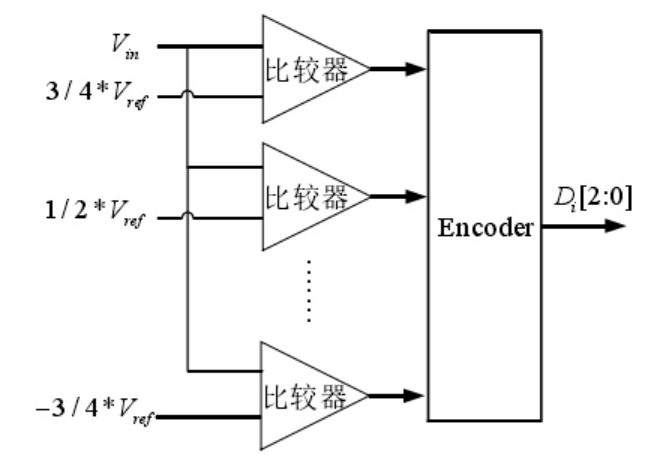
\includegraphics[width=8cm]{sub-ADC}
        \caption{\label{fig:sub-ADC}sub-ADC电路结构图}
    \end{figure}
    \par sub-ADC电路对应输入输出关系如下:
    \begin{align}
        \left\{
            \begin{array}{l}
            {-V_{ref} \leq V_{in} \leq\frac{-3}{4}V_{r e f},\ D_{i}=000} \\
            { -\frac{3}{4}V_{ref} \leq V_{in} \leq -\frac{1}{2}V_{ref},\ D_{i}=001} \\
            { -\frac{1}{2}V_{ref} \leq V_{in} \leq -\frac{1}{4}V_{ref},\ D_{i}=010} \\
            \cdots \\
            { \frac{3}{4}V_{ref} \leq V_{in} \leq V_{ref},\ D_{i}=110}
        \end{array}\right.
    \end{align}
    
\subsubsection{MDAC电路}
    MDAC电路采用电荷重分配型结构,以图2.5的1.5bit/级MDAC为例,电路中包含采样电容$ C_{s,i} $
    和反馈电容$ C_f $,同时有两组开关,分别由非交叠时钟$ k_1,\ k_2 $控制。$ k_1 $导通,$ k_2 $
    关断时,MDAC处于采样阶段;$ k_1 $关断,$ k_2 $导通时,MDAC处于放大阶段。其中,$ k_{1a},\ k_{2a} $
    提前关断,以减轻电荷注入效应。
    \begin{figure}[ht]
        \centering
        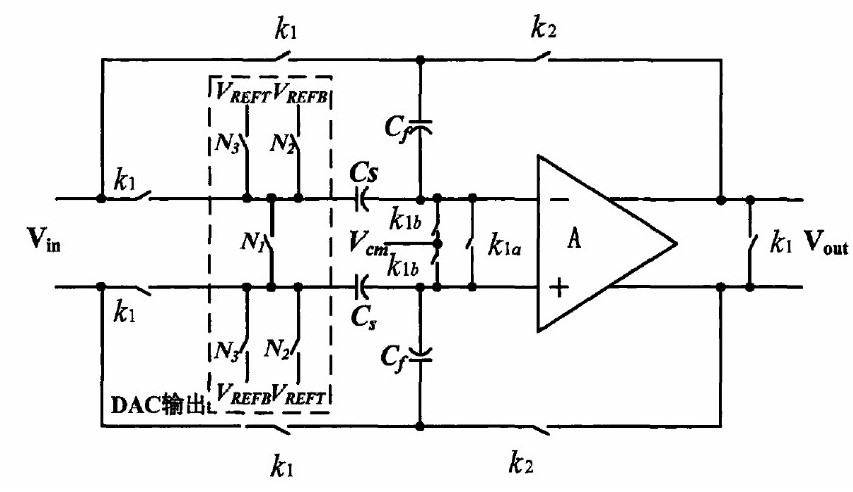
\includegraphics[width=10cm]{MDAC}
        \caption{\label{fig:MDAC}MDAC电路结构图}
    \end{figure}
    \par 处于采样阶段时,X点总电荷为: \\
    \begin{align}
        Q_{sample1}=\left(V_{X}-V_{in}\right)C_s
    \end{align}
    \par 当进入放大阶段时,则有: \\
    \begin{align}
        Q_{sample2}= -V_{out}C_f - DV_{ref}C_s
    \end{align}
    \par 由电荷守恒定律: \\
    \begin{align}
        V_{out} = V_{in}\frac{C_f+C_s}{C_f} - DV_{ref}\frac{C_s}{C_f}
    \end{align}
    \par 其中,$ DV_{ref} $的取值如图2.6,D为sub-ADC输出的编码:\\
    \begin{figure}[ht]
        \centering
        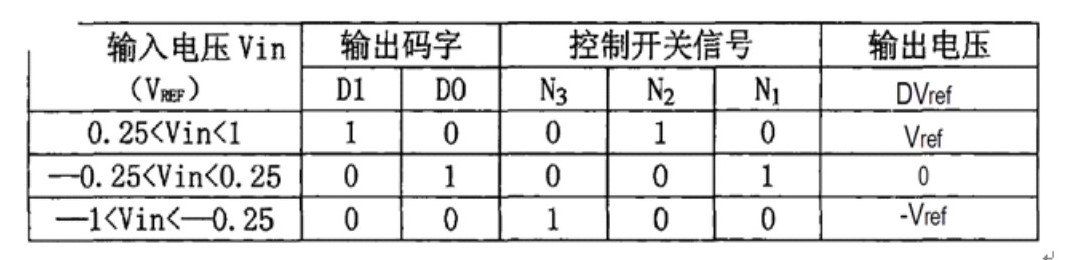
\includegraphics[width=10cm]{VREF}
        \caption{\label{fig:VREF}1.5bit/级MDAC参考电压与输入电压对应关系}
    \end{figure}
    \par 最终,可以得到输入输入电压与输出电压的函数关系: \\
    \begin{align}
        V_{\text {out}}=
        \left\{
            \begin{array}{ccc}{2 V_{\text {in}}-V_{\text {ref}}} & {\frac{V_{\text {ref}}}{4}<V_{i n}<V_{\text {ref}}} & {D_1D_0:10} \\
             {2 V_{\text {in}}} & {-\frac{V_{\text {ref}}}{4} \leq V_{\text {in}} \leq \frac{V_{\text {ref}}}{4}} & {D_1D_0:01} \\
             {2 V_{\text {in}}+V_{\text {ref}}} & {-V_{\text {ref}}<V_{\text {in}}<-\frac{V_{\text {ref}}}{4}} & {D_1D_0:00}
            \end{array}
        \right.
    \end{align}
    
    \begin{figure}[H]
        \centering
        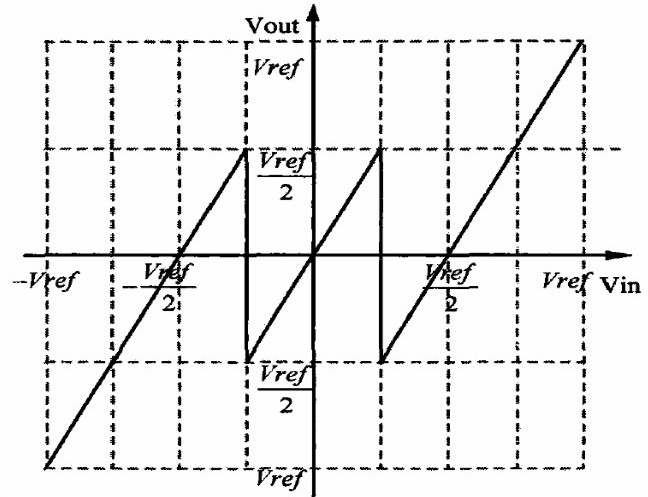
\includegraphics[width=8cm]{MDAC_inout}
        \caption{\label{fig:MDAC_inout}1.5bit/级MDAC传输曲线}
    \end{figure}

\subsection{数字校正技术}
    数字校正技术是流水线ADC中最基本的关键技术,由于各级的比较器速度快,不可避免地将产生比低速ADC
    更大的误差,使得余量放大后的输出超过量化范围,如\autoref{fig:os_error}。
    \begin{figure}[H]
        \centering
        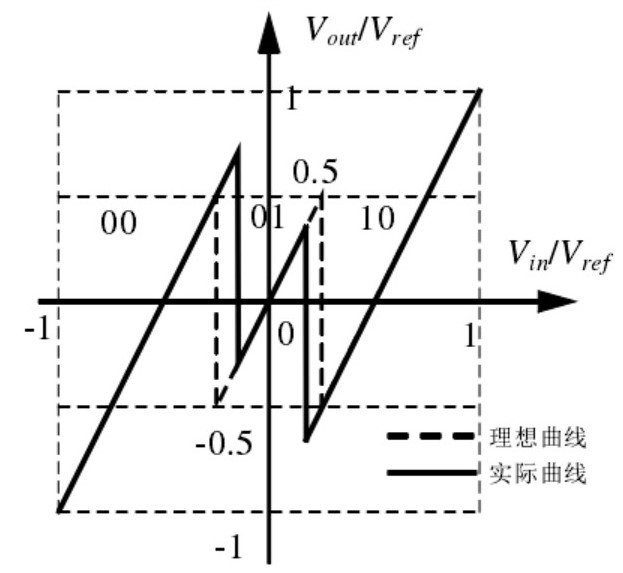
\includegraphics[width=10cm]{os_error}
        \caption{\label{fig:os_error}1.5bit/级MDAC的非理想传输曲线}
    \end{figure}
    流水线ADC冗余位数字校正技术由Stephen H Lew等人
    于1992年首次提出。这种校正算法利用错位相加的方法,将每一级多余的0.5bit用于校正误差。
    由于校正技术的存在,使的流水线ADC对比较器精度的要求大大下降,可以进一步提升运算速度、
    降低功耗。
    \par 下面继续利用\autoref{fig:os_error}来分析校正方法的原理。如果比较器在$ -\frac{V_{ref}}{4} $
    处产生$ \delta < \frac{V_{ref}}{4} $的误差,假设输入电压为$ V_{in,k} \in (-\frac{V_{ref}}{4},\ -\frac{V_{ref}}{4}+\delta) $,
    理想情况下,量化数字码为$ D_1^*D_0^* = 01 $,输出余量$ V_{in,k+1} = V_{out,k} \in (-\frac{V_{ref}}{2},\ 0) $。
    此时,若$ V_{in,k+1} \in (-\frac{V_{ref}}{2},\ -\frac{V_{ref}}{4}) $,下一级量化数字码为$ D_1^*D_0^* = 00 $,
    若$ V_{in,k+1} \in (-\frac{V_{ref}}{4},\ 0) $,下一级量化数字码为$ D_1^*D_0^* = 01 $,
    因此,第k级与第k+1级得到数字码为010或011.
    而实际量化数字码为$ D_1^*D_0^* = 00 $,输出余量$ V_{out} \in (\frac{V_{ref}}{2},\ V_{ref}) $,
    此时,下一级量化数字码为$ D_1^*D_0^* = 10 $,第k级与第k+1级得到数字码为010,与理想有最后一位误差,
    能够继续往下一级传递,前面误差均被抵消直到最后。由于到最后一级,误差已经很小,
    而且最后一级精度较高,因此误差可以忽略。

\section{12位SHA-less架构流水线ADC的系统设计}

\subsection{采样保持电路中的非理想因素}
    \subsubsection{热噪声}
    热噪声是电路噪声的主要来源,主要分为来自开关电容的热噪声和运算放大器的热噪声。
    \begin{figure}[H]
        \centering
        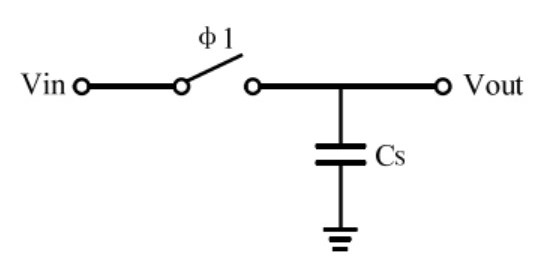
\includegraphics[width=10cm]{switch}
        \caption{\label{fig:switch}简单的采样开关电路}
    \end{figure}
    \par 以简单的采样开关电路为例,如\autoref{fig:switch}。当开关导通时,MOS管对应
    的导通电阻将会产生随机热噪声,开关断开后,采样电容上便储存了热噪声。由于电阻热噪声
    是随机变化的,没有办法进行校正,但是可以估算其热噪声的功率。假设MOS管导通电阻为
    $ R $,则其引入的热噪声功率谱密度为: \\
    \begin{align}
        S(f)=4kTR
    \end{align}
    \par 对功率谱积分得到其总噪声功率:\\
    \begin{equation}
        \begin{split}
            P_{n\_\text {tolal}} & =\int_{0}^{+\infty} \bar{V}_{n, c}^{2}(f)df\\
            & =\int_{0}^{+\infty} 4 k_{B} T R\left|\frac{1}{1+j \omega R C}\right|^{2} d\left(\frac{\omega}{2 \pi}\right) \\
            & = \frac{kT}{C_s}
        \end{split}
    \end{equation}
    \par 如\autoref{fig:kTnoise},在simulink环境下可以利用随机波形与总噪声幅度$ \sqrt{\frac{kT}{C_s}} $
    相乘,得到其噪声模型。
    \begin{figure}[H]
        \centering
        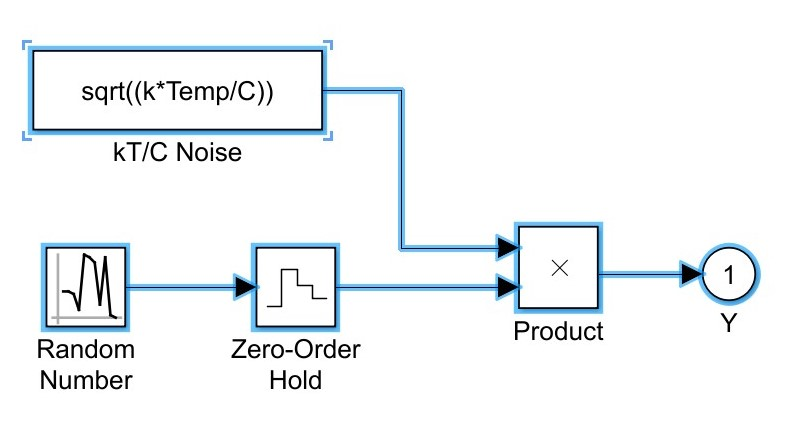
\includegraphics[width=10cm]{kTnoise}
        \caption{\label{fig:kTnoise}开关热噪声行为级仿真}
    \end{figure}
    \par 考虑到在高速低功耗流水线ADC中,为降低电路功耗,电容值一般为$ 10^{-12} $级别,其单个开关电路
    热噪声较小,可以视作忽略。
    \par 运放的热噪声主要是MOS管的沟道噪声,根据MOS管小信号等效模型,可以推导出运放噪声功率:\\
    \begin{align}
       P_{n,opa} \propto \frac{kT}{C_T}
    \end{align}
    \par $ C_T $为运放总等效输出电容。
    \par 如\autoref{fig:Opnoise},在simulink环境下可以利用随机波形与总噪声幅度$ \sqrt{\frac{kT}{C_s}} $
    相乘,得到其噪声模型,通过调节运放的增益delta,可以调节噪声的大小。
    \begin{figure}[H]
        \centering
        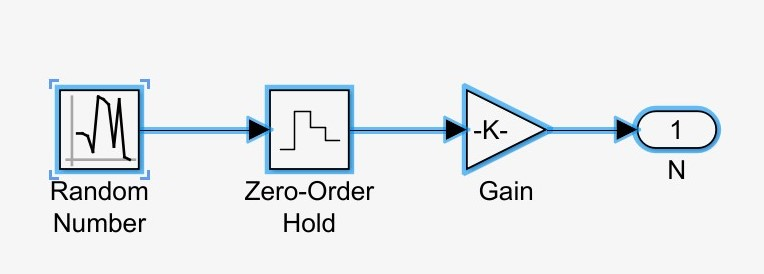
\includegraphics[width=10cm]{Opnoise}
        \caption{\label{fig:Opnoise}运放热噪声行为级仿真}
    \end{figure}
    \par 设置delta = 0.01,可以得到如\autoref{fig:Opnoise_com}的噪声:
    \begin{figure}[H]
        \centering
        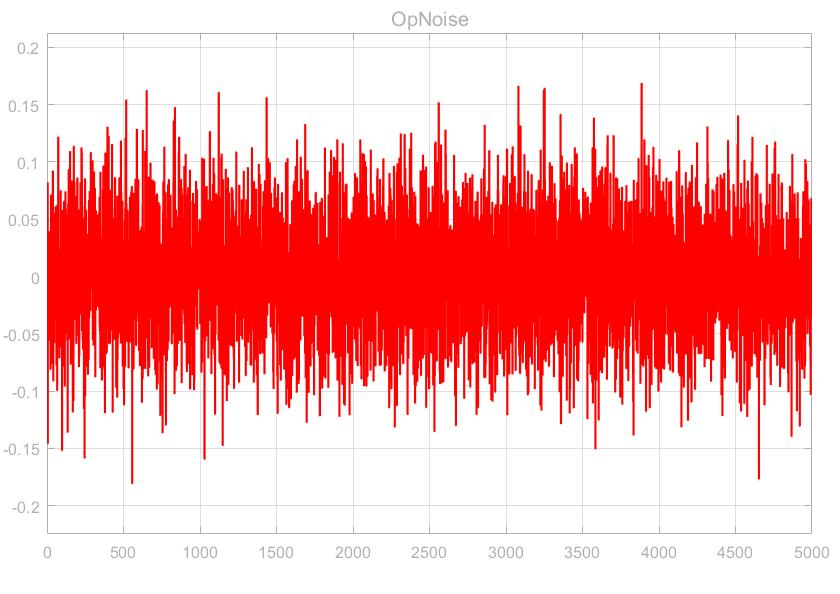
\includegraphics[width=10cm]{Opnoise_com}
        \caption{\label{fig:Opnoise_com}运放热噪声仿真}
    \end{figure}
    \par 由此可见噪声大小与电路电容大小成反比,若要减小热噪声,可以增大电容,但是大电容
    又将增加功耗和电路大小。在流水线ADC中,S/H电路集成了较多的开关电容,如\autoref{fig:SH},是
    电路热噪声的主要来源。为减小其噪声,不得不增大电容值,从而牺牲了电路的功耗和大小。
    于是,这也是论文提出SHA-less架构的主要原因。
    \begin{figure}[H]
        \centering
        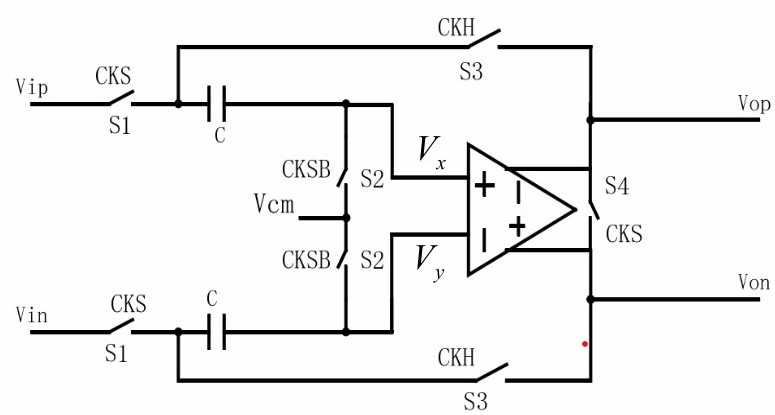
\includegraphics[width=10cm]{SH}
        \caption{\label{fig:SH}电容翻转型S/H电路}
    \end{figure}
    
    \subsubsection{传统的带S/H电路ADC}
    在实际的S/H电路中,还有时钟抖动引起的噪声,设输入信号为$ f(t) $,则
    \begin{align}
        \epsilon & = f(t+\Delta t)-f(t) \\
        V_{in}(t) & = V_{in,ideal}(t) + \frac{dV_{in}(t)}{dt}\Delta t 
    \end{align}
    如\autoref{fig:jitter}所示,在simulink中可以搭建模型对时钟抖动现象进行仿真,
    利用随机数生成器与输入信号瞬时斜率相乘,再进行输出。通过调节运放的增益delta,可以
    调节噪声的大小。
    \begin{figure}[H]
        \centering
        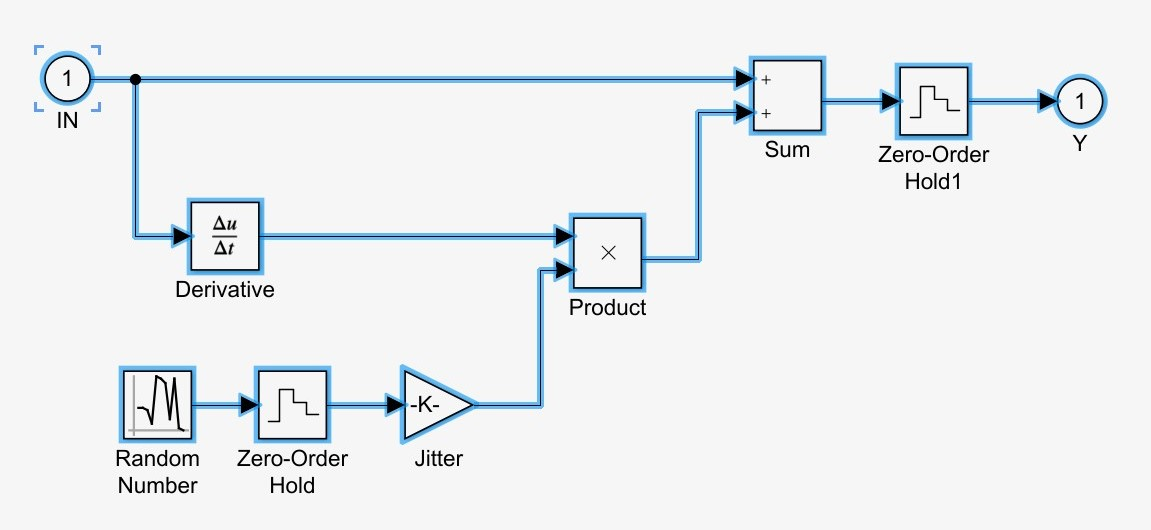
\includegraphics[width=10cm]{jitter}
        \caption{\label{fig:jitter}时钟抖动噪声行为级模型}
    \end{figure}
    \par 设置delta = 0.01,输入信号为正弦波,可以得到如\autoref{fig:jitter_com}波形:
    \begin{figure}[H]
        \centering
        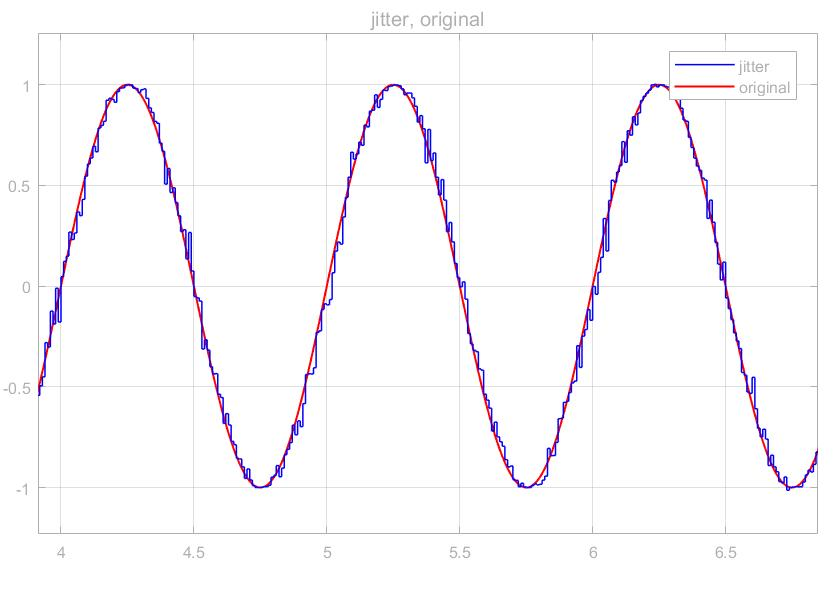
\includegraphics[width=10cm]{jitter_com}
        \caption{\label{fig:jitter_com}时钟抖动噪声对输入信号影响}
    \end{figure}
    \par 同时,S/H电路中的运算放大器工作在闭环模式,由于实际运放增益$ A_v \neq \infty $,
    则运放的闭环增益将会存在一定非线性误差
    \begin{align}
        \epsilon & = V_{in}\frac{1}{\beta A_v} \\
        V_{out} & = V_{in}\frac{A_v}{1+\beta A_v}
    \end{align}
    其中,$ \beta $为电路反馈系数,$ A_v $为运放开环增益。
    \par 如\autoref{fig:gainerror}所示,在simulink中利用函数模块Fcn可以大致实现运放增益误差模型,
    将误差近似为$ V_{out} = V_{in}\frac{1}{1+\frac{1}{\beta A_v}} $
    \begin{figure}[H]
        \centering
        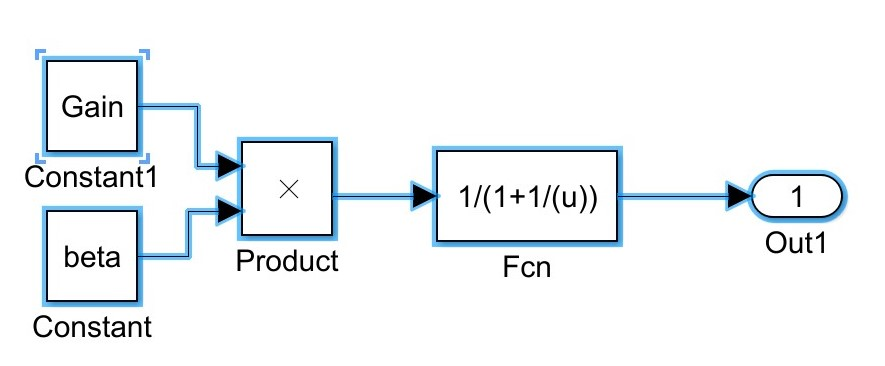
\includegraphics[width=10cm]{gainerror}
        \caption{\label{fig:gainerror}运放闭环增益误差行为级模型}
    \end{figure}

    \par 此外,由于实际运放单位增益带宽并非无穷大,将导致输出信号不完全建立。
    可以将S/H电路近似为单极点系统,当输入信号为$ \delta(t) $时,
    系统函数为
    \begin{align}
        H(s) = \frac{1}{1+\frac{s}{\beta\times GBW}}
    \end{align}
    其中,GBW为运放单位增益带宽,$ \beta $为电路反馈系数。
    \par 如\autoref{fig:Hs}所示,在simulink中利用传输函数模块Transfer Fcn
    可以实现运放信号不完全建立的误差模型,
    \begin{figure}[H]
        \centering
        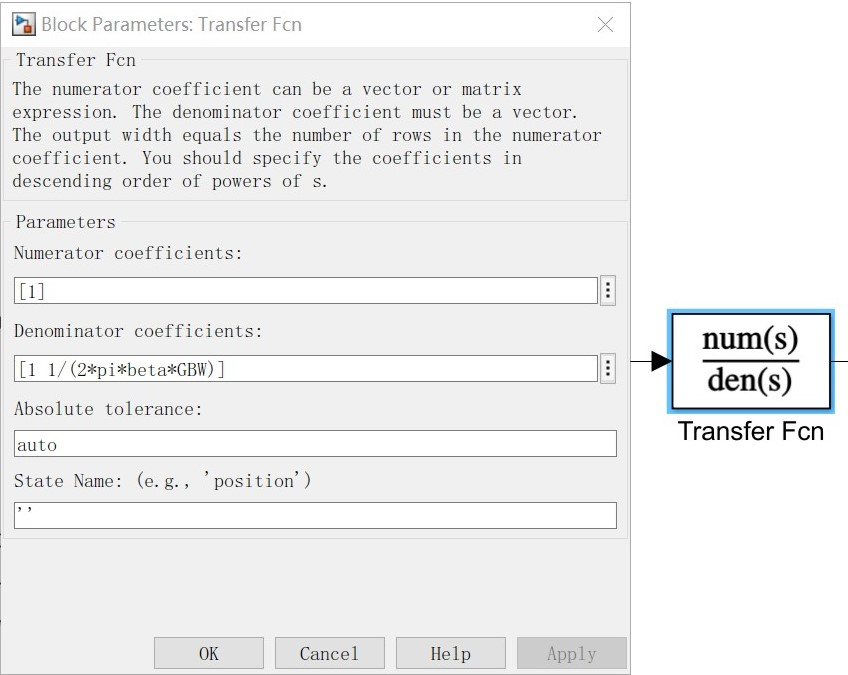
\includegraphics[width=10cm]{Hs}
        \caption{\label{fig:Hs}运放闭环增益误差行为级模型}
    \end{figure}


\subsection{带前端S/H电路ADC的行为级仿真}
    根据上述对S/H电路非理想性的分析,整合出同时考虑多种非理想因素的
    S/H电路simulink模型,如\autoref{fig:SH_sim1}所示。
    \begin{figure}[H]
        \centering
        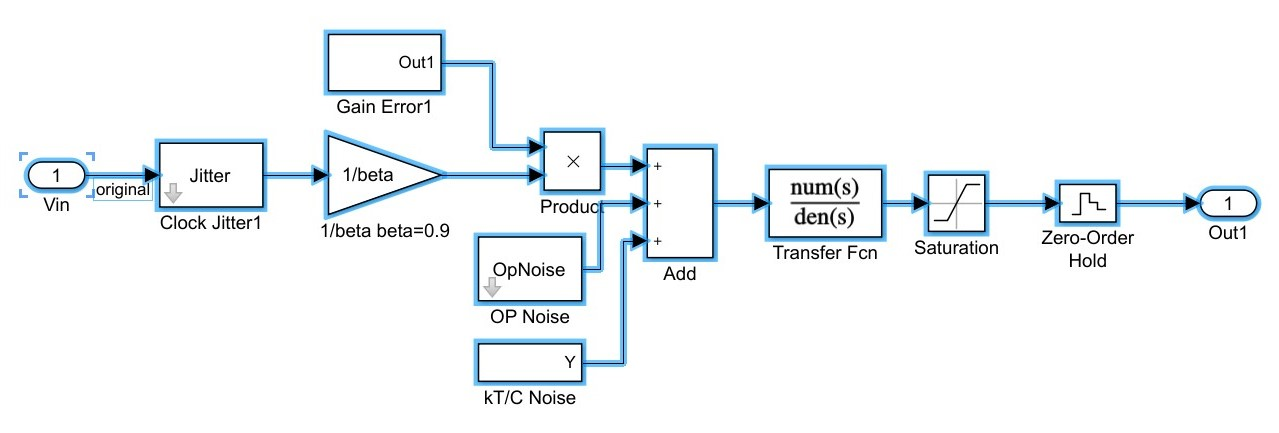
\includegraphics[width=10cm]{SH_sim1}
        \caption{\label{fig:SH_sim1}考虑非理想因素的S/H电路行为级模型}
    \end{figure}
    \par 如\autoref{fig:SH_mask},可以根据实际需要对S/H电路非理想因素进行调整。
    \begin{figure}[H]
        \centering
        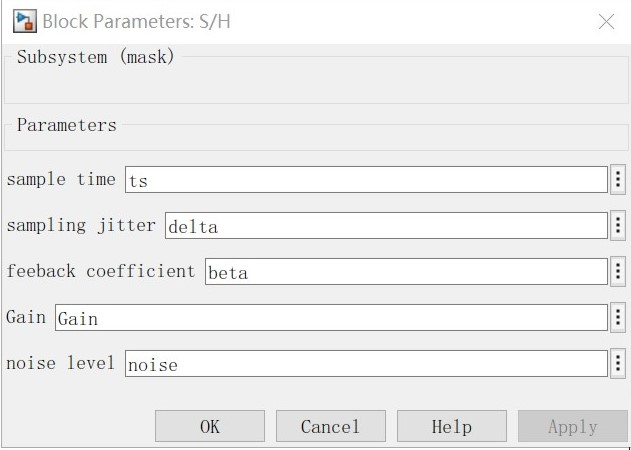
\includegraphics[width=10cm]{SH_mask}
        \caption{\label{fig:SH_mask}考虑非理想因素的S/H电路行为级模型}
    \end{figure}
    ts为采样时间,与仿真时的步长一致;delta为时钟抖动误差大小;beta为系统反馈系数;
    Gain为运放开环增益大小;noise为噪声功率水平。
    \par 为简化整体电路模型与难度,该模型仅用于前端S/H电路,对于
    子结构中的S/H,可认为其非理想因素较少,仅采用如\autoref{fig:SH_sim2}所示的
    S/H模型,只考虑时钟抖动噪声。
    \begin{figure}[H]
        \centering
        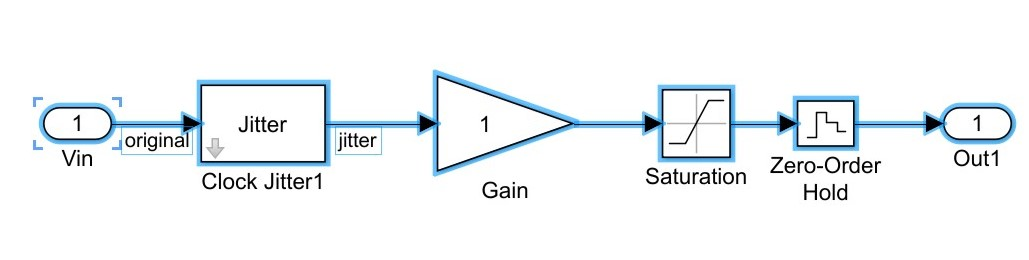
\includegraphics[width=10cm]{SH_sim2}
        \caption{\label{fig:SH_sim2}简化后的非理想S/H电路行为级模型}
    \end{figure}
    \par 由此,可以得到考虑非理想因素的流水线ADC('12\_bit\_pipeline\_adc.slx'),
    其中,S/H电路的使用如\autoref{fig:with_SH1}和\autoref{fig:with_SH2}所示
    \begin{figure}[H]
        \centering
        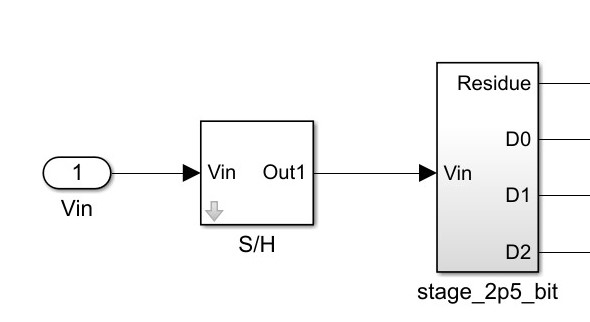
\includegraphics[width=10cm]{with_SH1}
        \caption{\label{fig:with_SH1}前端S/H电路}
    \end{figure}
    \begin{figure}[H]
        \centering
        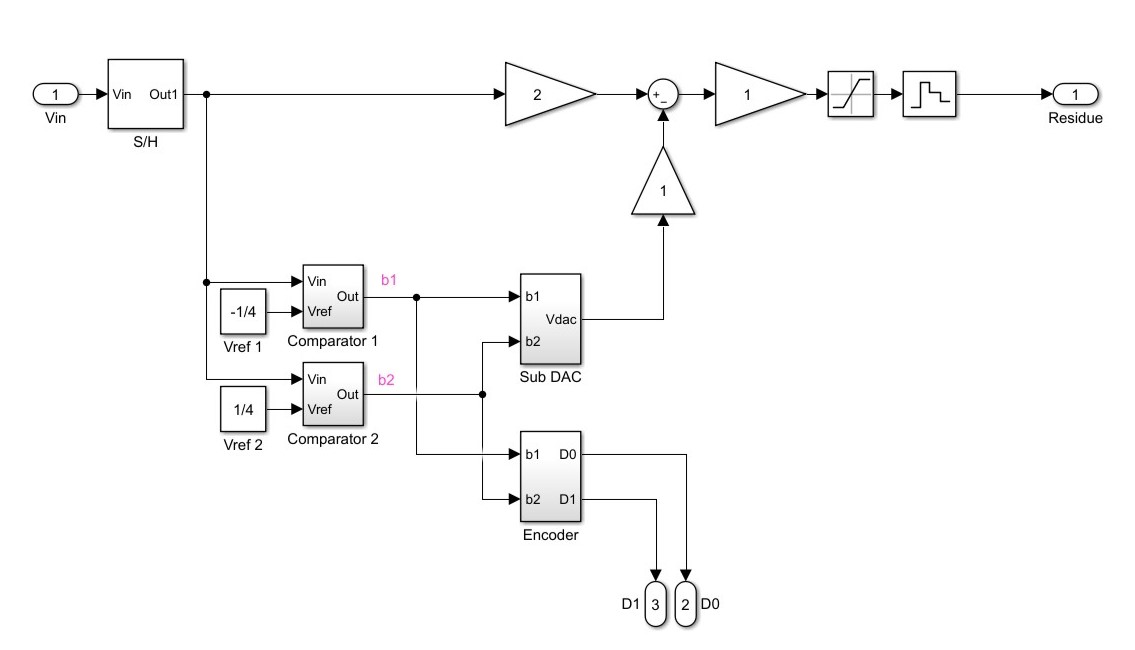
\includegraphics[width=10cm]{with_SH2}
        \caption{\label{fig:with_SH2}子结构中S/H电路}
    \end{figure}
    \par 仿真结果如\autoref{fig:ADC_out1}和\autoref{fig:ADC_spectrum1}所示,
    仿真结果显然不尽人意,相比于完全理想的流水线ADC(SNDR=73.73dB, ENOB=11.95),
    在考虑诸多非理想性后性能有了明显的下降,信噪失真比SNDR仅9.92dB,有效位数ENOB仅1.36
    \begin{figure}[H]
        \centering
        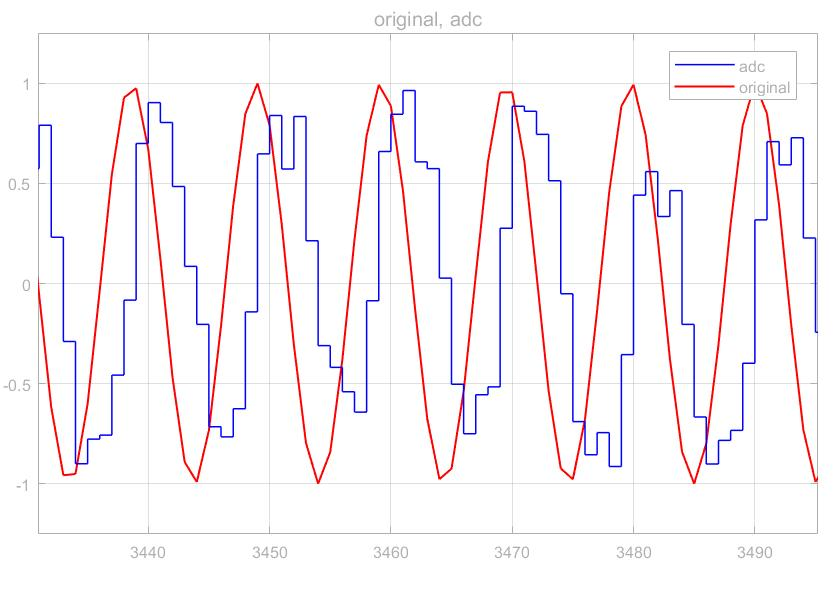
\includegraphics[width=8cm]{ADC_out1}
        \caption{\label{fig:ADC_out1}传统流水线ADC输出}
    \end{figure}
    \begin{figure}[H]
        \centering
        \includegraphics[width=8cm]{ADC_spectrum1}
        \caption{\label{fig:ADC_spectrum1}传统流水线ADC频谱}
    \end{figure}

\subsection{SHA-less架构ADC的行为级仿真}
    去除前置S/H电路的结构称作SHA-less架构,这样能够大大减少S/H电路中非理想因素对
    流水线ADC的影响,同时可以降低功耗(约20\%~30\%),满足当下ADC设计的要求。由于第一级子结构的
    输入信号变为了直接输入而不是采样信号,这直接导致了MDAC与sub-ADC处理的信号可能存在不一致现象,
    也被称作孔径误差。一般的解决方案是利用开关电容对MDAC的输入端和sub-ADC的输入端进行分别采样,
    利用数字校正技术予以校正。
    \par 为了验证SHA-less结构是否拥有优越性,在simulink下进行仿真。将上一小节中的前端S/H电路去除
    后,可以得到如\autoref{fig:ADC_out2}和\autoref{fig:ADC_spectrum2}仿真结果
    \begin{figure}[H]
        \centering
        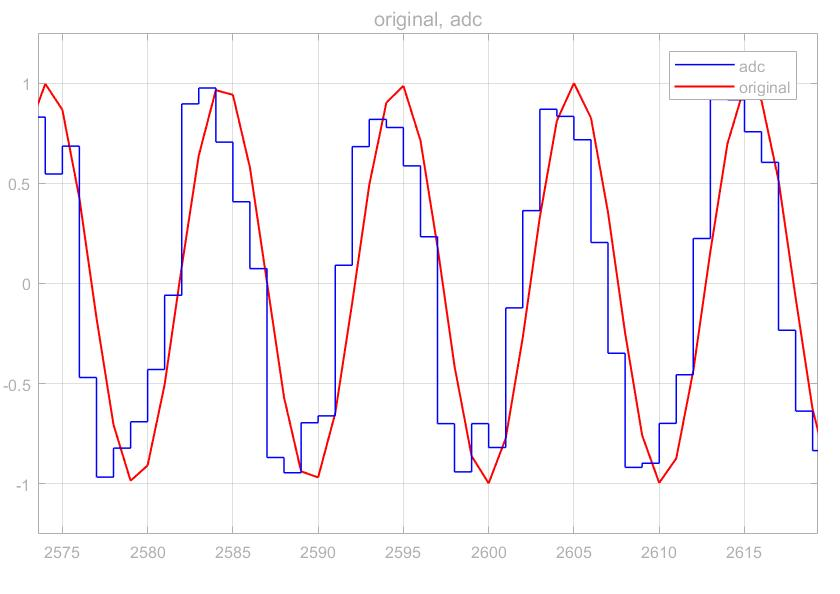
\includegraphics[width=10cm]{ADC_out2}
        \caption{\label{fig:ADC_out2}SHA-less流水线ADC输出}
    \end{figure}
    \begin{figure}[H]
        \centering
        \includegraphics[width=10cm]{ADC_spectrum2}
        \caption{\label{fig:ADC_spectrum2}SHA-less流水线ADC频谱}
    \end{figure}
    \par 由于有大量非理想因素的存在,性能并没有非常大的提升,但是对比上一节的结果如\autoref{tab:SHA_com},
    可以发现SHA-less电路在高速低功耗流水线ADC中有用武之地。
    \begin{table}[ht]
        \centering
        \caption{\label{tab:SHA_com}SHA-less架构参数对比}
        \begin{tabular}{|c|c|c|}
            \hline
            种类 & 传统ADC & SHA-less \\ \hline
            SNDR(dB) & 9.92 & 13.56 \\ \hline
            ENOB & 1.36 & 1.96   \\ \hline
        \end{tabular}
    \end{table}


\section{关键技术以及电路设计仿真}
\subsection{运算放大器}
    \subsubsection{电路设计方程}
    各参数的设计方程如下:
    \begin{align}
        & C_c \geq 0.22C_L \\
        & \frac{g_{m6}}{g_{m2}} > 10 \\
        & GBW = \frac{g_{m1}}{C_c} \\
        & SR \approx \frac{I_{M5}}{C_c} \\
        & A_{v1} = -\frac{g_{m1}}{g_{ds2}+g_{ds4}} \\
        & A_{vc} = -\frac{g_{ds5}}{2g_{m3}} \\
        & CMRR = \frac{A_{v1}}{A_{vc}} = \frac{2g_{m3}}{g_{ds5}(g_{ds2}+g_{ds4})} \\
        & A_{v2} = -\frac{g_{m6}}{g_{ds6}+g_{ds7}} \\
        & A_v = A_{v1}A_{v2} = \frac{g_{m1}g_{m6}}{(g_{ds2}+g_{ds4})(g_{ds6}+g_{ds7})} \\
        & V_{cm,max} = V_{DD} - \sqrt{\frac{I_{M5}}{\beta_1}} - |V_{DS5,sat}| - max(|V_{TP1}|) \\
        & V_{cm,min} = V_{SS} + \sqrt{\frac{I_{M5}}{\beta_3}} + max(V_{TN3}) - min(|V_{TP1}|) \\
        & P=(V_{DD}-V_{SS})(I_{M5}+I_{M6}+I_R)
    \end{align}

    \subsubsection{计算MOS管参数}
    首先根据上一小节设计方程,计算各MOS管参数. \\
    \indent 利用导师提供的.08工艺进行计算:
    \begin{align*}
        & \mu_n C_{ox}=110\mu A/V^2 \ & \mu_pC_{ox}=50\mu A/V^2 \\
        & \lambda_n=0.04V^{-1} \ & \lambda_p=0.05V^{-1} \\
        & T_{ox}=14\times 10^{-9} \\
        & A_v>5000 \ & GB=5MHz \\ 
        & C_L=10pF & SR>10V/\mu s \\
        & ICMR: \ [-2V,\ 1V] \ & V_{out}=\pm 2V \\
        & V_{DD}=2.5V \ & V_{SS} = -2.5V \\
        & P_{diss} \leq 2mW \ & L = 1\mu m 
    \end{align*}
    \indent 从 (4-1) 可以得到: $ C_c \geq 2.2pF $, 令: 
    \begin{align}
        C_c = 3pF 
    \end{align}
    \indent 从 (4-4) 可以得到: $ I_{M5} \approx C_cSR $, 令: 
    \begin{align} 
        I_{M5} = 30\mu A 
    \end{align}
    \indent 从 (4-10) 可以得到: 
    \begin{align}
        V_{cm,min} & =-2V\\
        max(|V_{TN3}|) & =0.85V\\
        min(|V_{TP1)}| & =0.55V
    \end{align}
    \begin{align}
        (\frac{W}{L})_3 = \frac{I_{M5}}{\mu_nC_{ox}(-V_{SS} + V_{cm,min} - max(|V_{TN3}|) + min(|V_{TP1}|))^2}
    \end{align}
    \par 因此
    \begin{align} 
        (\frac{W}{L})_3 = \frac{30\times 10^{-6}}{(110\times 10^{-6})[2.5-2-0.85+0.55]^2} = 6.82 
    \end{align}
    \indent 令: 
    \begin{align} 
        (\frac{W}{L})_3 = (\frac{W}{L})_4 = 7  
    \end{align}
    \indent 从 (4-3) 可以得到: 
    \begin{align} 
        g_{m1} = 94.2478\mu S 
    \end{align}
    \indent 从 $ g_{m1} = 2\sqrt{\frac{\mu_pC_{ox}}{2}(\frac{W}{L})_1I_{M1}} $ 和 $ I_{M1} = I_{M2} = \frac{I_{M5}}{2} $ 可以得到:\\
    \begin{align} 
        (\frac{W}{L})_1 = (\frac{W}{L})_2 = 5.92 
    \end{align}
    \indent 令: 
    \begin{align} 
        (\frac{W}{L})_1 = (\frac{W}{L})_2 = 6 
    \end{align}
    \indent 从 (4-10) 可以得到: $ V_{DS5,sat} = V_{DD} - V_{cm,max} - \sqrt{\frac{I_{M5}}{\beta_1}} - max(|V_{TP1}|) $,
    和 $ V_{DD}=2.5V, V_{cm,max} = 1V, max(|V_{TP1}|) = 0.85V $, 因此有: \\
    \begin{align} 
        V_{DS5,sat} = 2.5 - 1 - \sqrt{\frac{30\times 10^{-6}}{6\times 50\times 10^{-6}}} - 0.85 = 0.334V 
    \end{align}
    \indent 从 $ I_{M5} = \frac{\mu_pC_{ox}}{2}(\frac{W}{L})_5(V_{GS5}-V_{TN5})^2 $, 可得: \\
    \begin{align} 
        (\frac{W}{L})_5 = \frac{2\times 30\times 10^{-6}}{50\times 10^{-6}\times0.334^2} = 10.77 
    \end{align}
    \indent 令: 
    \begin{align} 
        (\frac{W}{L})_5 = 11 
    \end{align}
    \indent 从 (4-2) 可得:
    \begin{align} 
        g_{m6} \geq 942.478\mu S 
    \end{align}
    \indent 令: 
    \begin{align} 
        g_{m6} = 943\mu S
    \end{align}
    \indent 从 $ g_{m4} = 2\sqrt{\frac{\mu_nC_{ox}}{2}(\frac{W}{L})_4I_{M4}} $ and $ I_{M4} = \frac{I_{M5}}{2} $ 可以得到:\\
    \begin{align} 
        g_{m4} = 2\sqrt{\frac{110\times 10^{-6}}{2}\times 7\times 15\times 10^{-6}} = 151.9868 \mu S 
    \end{align}
    \indent 在直流工作状态下,差分放大器的左右电路对称 因此 $ V_{GS4} = V_{GS6} $, then: \\
    \begin{align} 
        (\frac{W}{L})_6 = (\frac{W}{L})_4\frac{g_{m6}}{g_{m4}} = 43.43 
    \end{align}
    \indent 令:
    \begin{align} 
        (\frac{W}{L})_6 = 44 
    \end{align}
    \indent 从  $ g_{m6} = 2\sqrt{\frac{\mu_nC_{ox}}{2}(\frac{W}{L})_6I_{M6}} $, we have: \\
    \begin{align} 
        I_{M6} = I_{M7} = 91.8646\mu A 
    \end{align}
    \indent 因此: 
    \begin{align} 
        (\frac{W}{L})_7 = (\frac{W}{L})_5\frac{I_{M7}}{I_{M5}} = 33.68 
    \end{align}
    \indent 令:
    \begin{align} 
        (\frac{W}{L})_7 = 34 
    \end{align}
    \indent 最终, 令偏置电流 $ I_R = I_{M5} $, 则: 
    \begin{align} 
        (\frac{W}{L})_9 = (\frac{W}{L})_5 = 11 
    \end{align}
    \begin{table}[H]
        \centering
        \begin{tabular}{|c|c|c|}
        \hline
        MOS & $ \frac{W}{L} $ & $ I(\mu A) $ \\ \hline
        $ M_1,\ M_2 $ & $ 6 $ & $ 15 $ \\ \hline
        $ M_3,\ M_4 $ & $ 7 $  & $ 15 $ \\ \hline
        $ M_5,\ M_9 $ & $ 11 $ & $ 30 $ \\ \hline
        $ M_6 $ & $ 44 $ & $ 92 $ \\ \hline
        $ M_7 $ & $ 34 $  & $ 92 $ \\ \hline
        \end{tabular}
        \caption{各MOS管宽长比以及电流}
    \end{table}

    至此,可以利用HSPICE对运算放大器进行仿真\\
    \subsubsection{开环测试}
    令共模输入为 0V, 差分输入接到正极输入,以此来进行直流仿真。各MOS管的直流工作点如\autoref{fig:direct}: \\
    \begin{figure}[H]
        \centering
        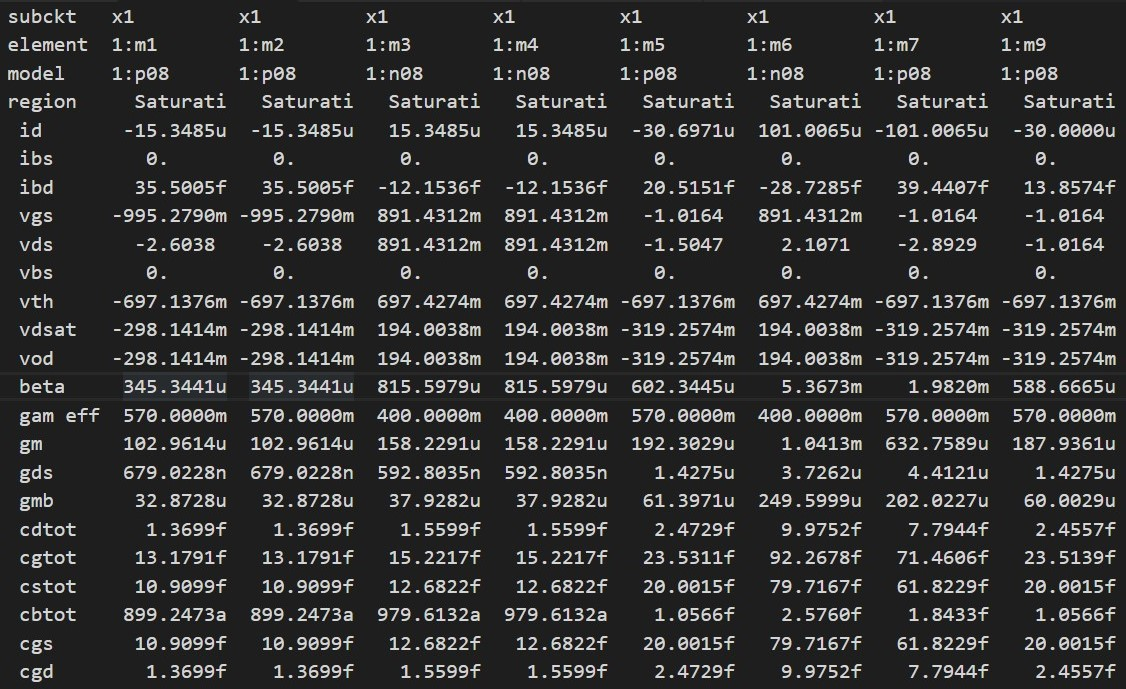
\includegraphics[width=16cm]{/project1/openloop_biaspoint.jpg}
        \caption{\label{fig:direct}各MOS管直流工作点}
    \end{figure}
    \indent 所有的MOS管都工作在饱和区,均正常工作。 \\
    \indent 首先计算整体电路的功耗: \\
    \indent 对差分输入级: \\
    \centerline{$ P_{diff} = 5V\times 30.6971\mu A $} \\
    \indent 对共模输入级: \\
    \centerline{$ P_{comm} = 5V\times 101.0065\mu A $} \\
    \indent 对偏置电流: \\
    \centerline{$ P_{csc} = 5V\times 30\mu A $} \\
    \indent 电路总体功耗为: \\
    \centerline{$ P = 0.81mW $} \\
    \indent 满足 $ P_{diss} \leq 2mW $的要求 \\
    \indent 然后,根据参数估计运放的增益: \\
    \begin{align}
        A_{v1} = -\frac{g_{m2}}{g_{ds2}+g_{ds4}} & = -\frac{102.9614\mu}{679.0228n+592.8035n} = -80.96 \\
        A_{v1} = -\frac{g_m6}{g_{ds6}+g_{ds7}} & = -\frac{1.0413m}{3.7262\mu+4.4121\mu} = -127.95 \\
        A_v & = A_{v1}A_{v1} = 10359 = 80.31dB
    \end{align}
    \indent 如\autoref{fig:gain},为增益仿真结果: 
    \begin{figure}[H]
        \centering
        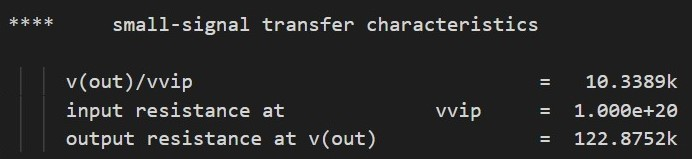
\includegraphics[width=10cm]{/project1/gain&res.jpg}
        \caption{\label{fig:gain}增益与输出电阻仿真结果}
    \end{figure}
    \indent 增益高达10k,满足 $ A_v \geq 5000 $ 的要求 \\
    \indent W利用MATLAB工具,如\autoref{fig:out}, 可以得到 $ V_{out} \in [-2.2292,\ 2.186] $ 
    满足输出电压范围的要求 $ V_{out} = \pm 2V $. \\ 
    \begin{figure}[H]
        \centering
        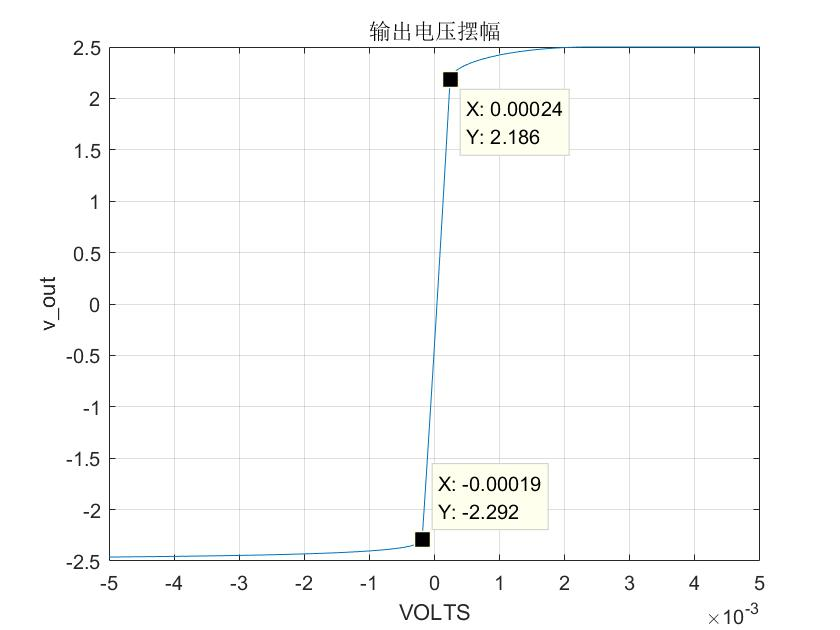
\includegraphics[width=12cm]{/project1/out.jpg}
        \caption{\label{fig:out}输出电压曲线}
    \end{figure}
    \indent 通过仔细观测输出电压曲线如\autoref{fig:os},可以进一步得到电路的偏置电压, 
    $ V_{in,os} = 40\mu V,\ V_{out,os} = -392.9mV $ \\
    \begin{figure}[H]
        \centering
        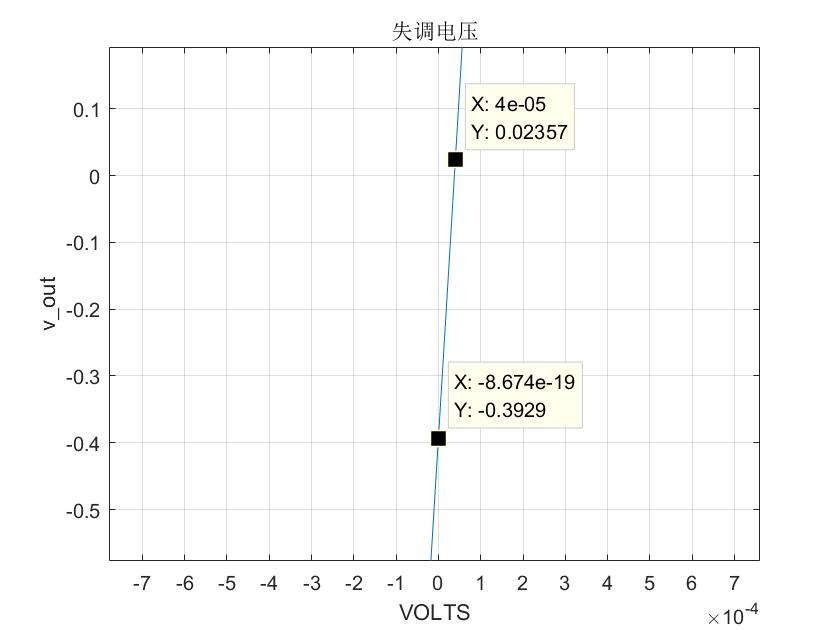
\includegraphics[width=10cm]{/project1/os.jpg}
        \caption{\label{fig:os}电路偏置电压}
    \end{figure}
    \indent 为了得到准确的增益,下面进行交流仿真,如\autoref{fig:ac}
    \begin{align}
        A_v & = 80.29dB = 10339 \\
        GBW & = 5.012MHz \\
        \phi & = 180-112.7 = 67.3^\circ \\
    \end{align} 
    \indent 上述均满足要求。\\ 
    \begin{figure}[H]
        \centering
        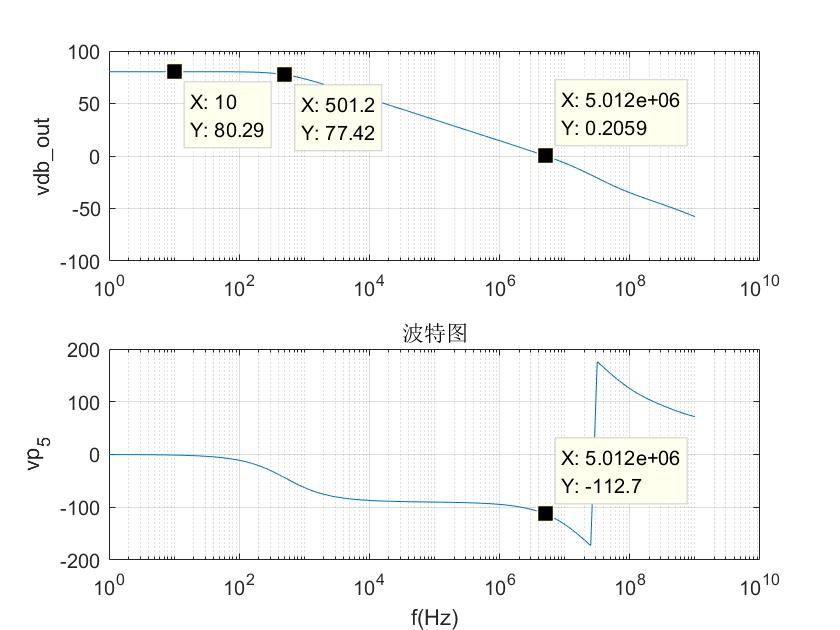
\includegraphics[width=10cm]{/project1/gain.jpg}
        \caption{\label{fig:ac}波特图}
    \end{figure}
    \subsubsection{单位增益测试}
    将运放接为反馈电路,使 $ \beta = 1 $,即电压跟随器结构。并得到如\autoref{fig:icmr},输入电压与输出电压和电流的关系\\
    \indent ICMR为: $ [-2.38V,\ 1.23V] $, 满足设计要求 $ [-1V,\ 2V] $ \\
    \begin{figure}[H]
        \centering
        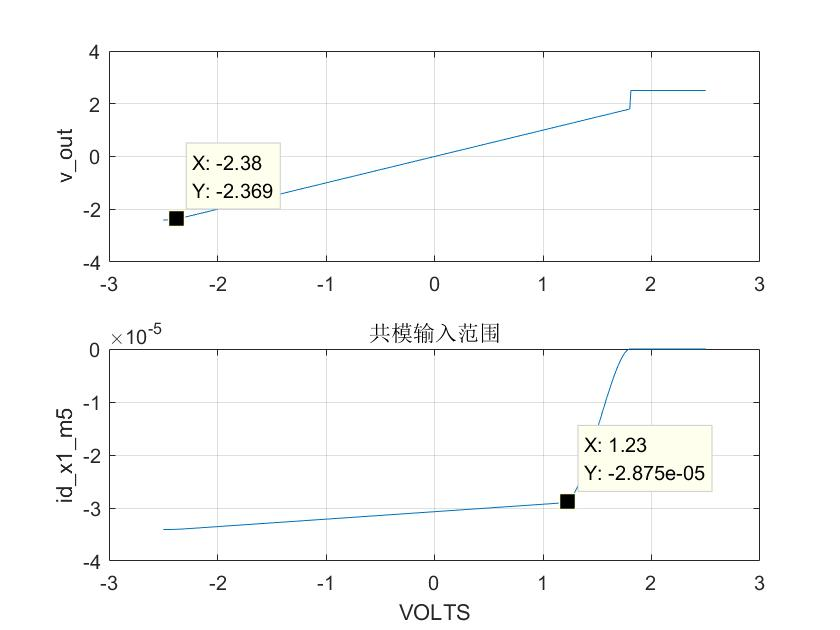
\includegraphics[width=10cm]{/project1/common_input.jpg}
        \caption{\label{fig:icmr}共模输入范围}
    \end{figure}
    \indent 此外,利用PWL信号输入可以测试压摆率,采用幅度为$ 4V $的大信号和幅度为$ 0.2V $的小信号。 \\
    \indent 从(4-10),可以计算 $ SR \approx \frac{I_{M5}}{C_c} = 10V/\mu s $ \\
    \indent 然而如\autoref{fig:SR1}和如\autoref{fig:SR2}大信号时的输出仅从$ -2V $ 到 $ 1.796V $,小信号时的输出仅从 $ -0.1001V $ 到 $ 0.09985V $ 
    \begin{align}
        SR_{up} & = \frac{1.543+1.575}{0.4981-0.07813} = 7.43V/\mu s \\
        SR_{down} & = \frac{1.482+1.568}{2.355-2.077} = 10.97V/\mu s 
    \end{align}
    \indent 上行压摆率$ SR_{up} $ 并未达到要求$ SR \geq 10V/\mu s $. \\
    \begin{figure}[H]
        \centering
        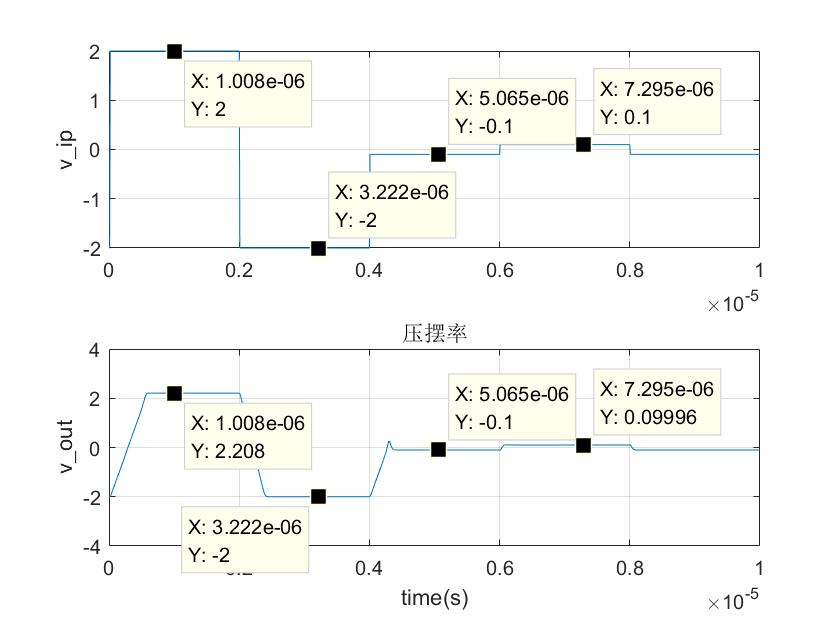
\includegraphics[width=10cm]{/project1/SR1.jpg}
        \caption{\label{fig:SR1}压摆率测试}
    \end{figure}
    \begin{figure}[H]
        \centering
        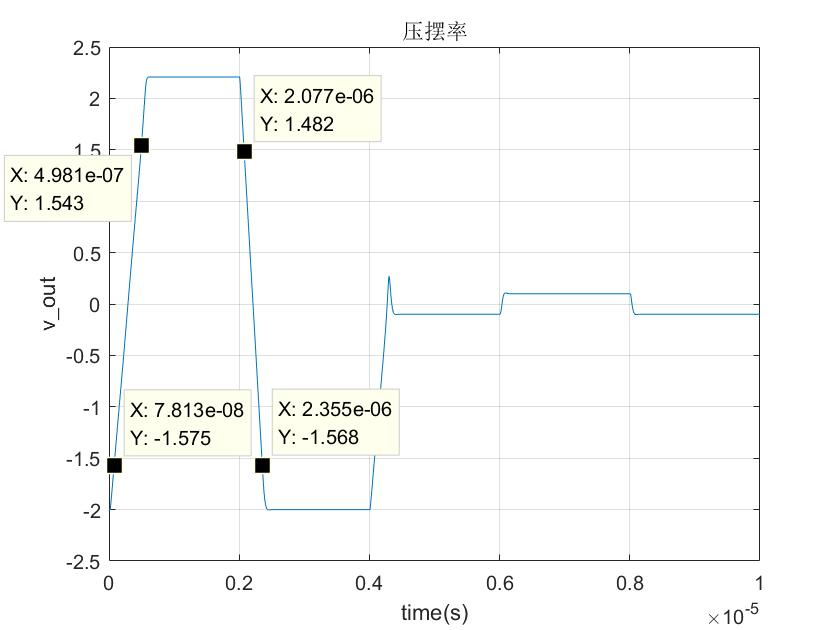
\includegraphics[width=10cm]{/project1/SR2.jpg} \\
        \caption{\label{fig:SR2}压摆率测试(放大)}
    \end{figure}
    \subsubsection{共模抑制比测试}
    将正负输入同时接到一个电压源,则 $ CMRR \approx \frac{v_{cm}}{v_o} $. \\
    \indent 如\autoref{fig:cmrr},可得: \\
    \centerline{$ CMRR = 84.82dB $} \\
    \begin{figure}[H]
        \centering
        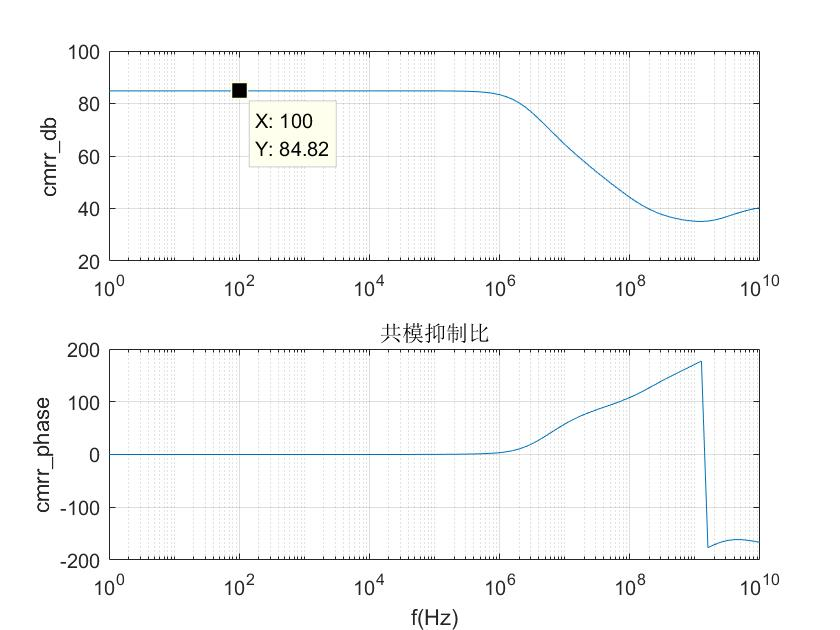
\includegraphics[width=10cm]{/project1/cmrr.jpg}
        \caption{\label{fig:cmrr}共模波特图}
    \end{figure}

    \indent 总体参数为: \\
    \begin{table}[H]
        \centering
        \begin{tabular}{|c|c|c|}
        \hline
        Parameters & Requirements & Result \\ \hline
        static power & $ \leq 2mW  $ & $ 0.81mW $ \\ \hline
        open loop gain & $ 73.98dB $ & $ 80.29dB $ \\ \hline
        GBW & $ 5MHz $ & $ 5.012MHz $ \\ \hline
        $\phi$ & $ \geq 60^\circ $ & $ 67.3^\circ $ \\ \hline
        SR & $ \geq 10V/\mu s $ & $ 7.43,\ 10.72(V/\mu s) $ \\ \hline
        CMRR & none & $ 84.82dB $ \\ \hline
        output voltage swing & $ [-2V,\ 2V] $ & $ [-2.2292V,\ 2.186V] $ \\ \hline
        ICMR & $ [-2V,\ 1V] $ & $ [-2.369V,\ 1.23V] $ \\ \hline
        \end{tabular}
        \caption{\label{tab:all}电路总体参数}
    \end{table} 
        \indent 尽管部分参数并未达到设计要求,但是应用在论文的流水线ADC中,
        该运放能够较好地完成任务

\subsection{开关电路}
在每一级子电路中,S/H电路以及MDAC均采用了开关电容电路,开关的选择
将会对电路性能造成一定程度的影响。
    \subsubsection{NMOS开关}
    NMOS开关是最简单的一种开关,利用MOS管通断的特性,通过控制
    G极的电压,即可控制MOS管通断。理想情况下,导通时NMOS导通电阻为0,
    然而在实际使用中,NMOS管工作在线性区,其等效电阻应为: 
    \begin{align}
        R_{on} = \frac{1}{\mu_nC_{ox}\frac{W}{L}(V_{GS}-V_{in}-V_{TN})}
    \end{align}
    \par 同时,其导通电阻与接入输出端的电容形成低通滤波器,导致信号经过开关
    时会产生一定的衰减与失真。同时由于G极输入电压不断变化,导致$ V_{GS} $不断
    变化,因而开关的导通电阻也在不断变化,使得开关整体性能不够稳定。
    \par 利用HSPICE仿真,可以得到NMOS开关的大致性能。
    如\autoref{fig:nmos}和\autoref{fig:nmos_d},可以发现其输出的误差较大,
    有明显的失真,并且夹杂较大的信号毛刺,容易对后续电路产生影响。
    \begin{figure}[H]
        \centering
        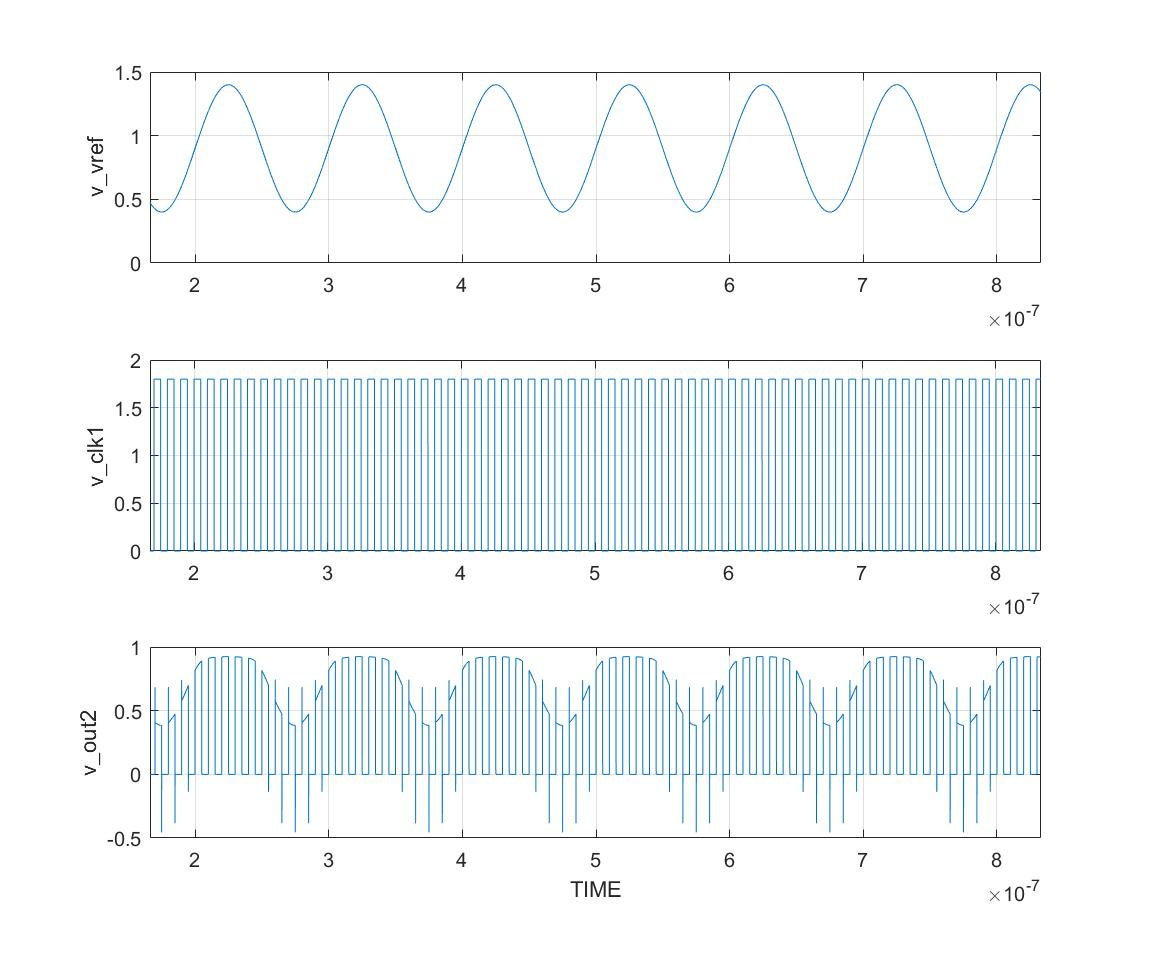
\includegraphics[width=8cm]{nmos}
        \caption{\label{fig:nmos}NMOS开关电路仿真}
    \end{figure}
    \begin{figure}[H]
        \centering
        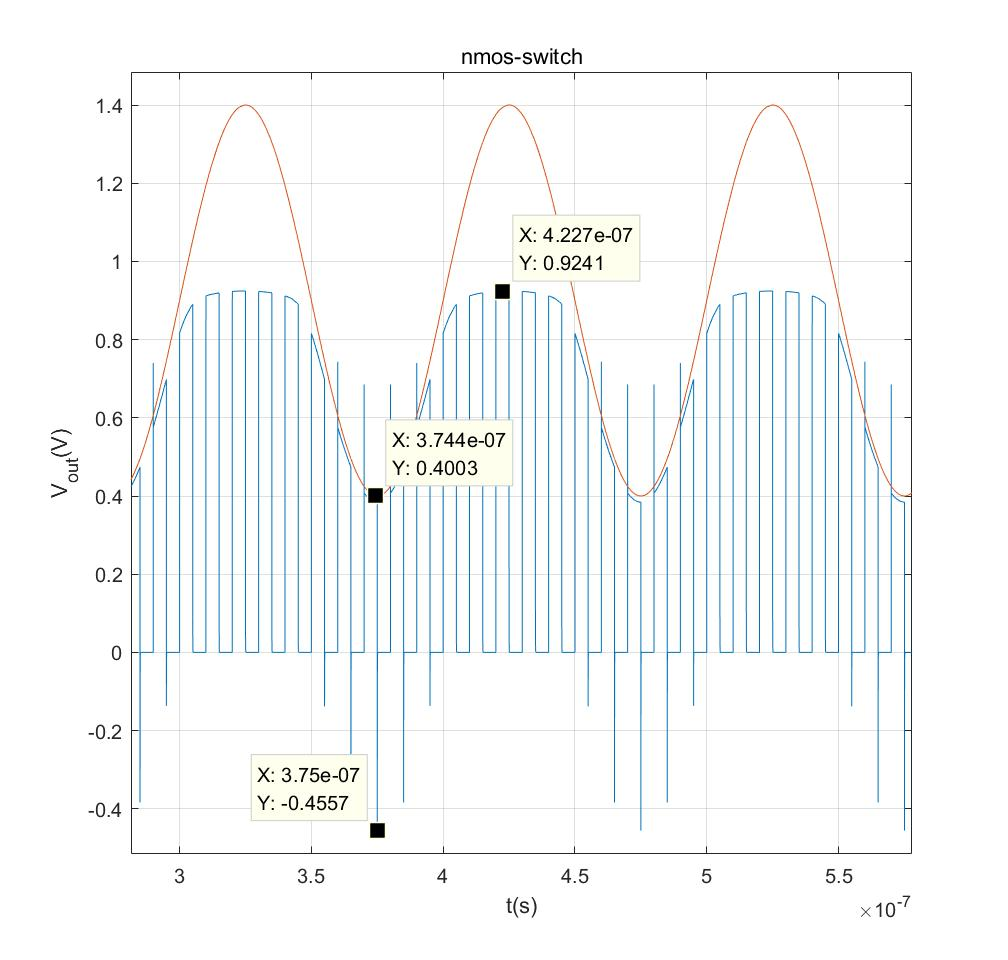
\includegraphics[width=8cm]{nmos_d}
        \caption{\label{fig:nmos_d}NMOS开关输出信号}
    \end{figure}

    \subsubsection{传输门开关(transmission-gate)}
    传输门开关利用NMOS与PMOS并联,如\autoref{fig:transmission-gate-n},
    由于NMOS管在输入电压较低时能够保持
    在线性区,PMOS在输入电压较高时能保持在线性区,利用二者的互补性,能够
    提高开关的性能。
    \begin{figure}[H]
        \centering
        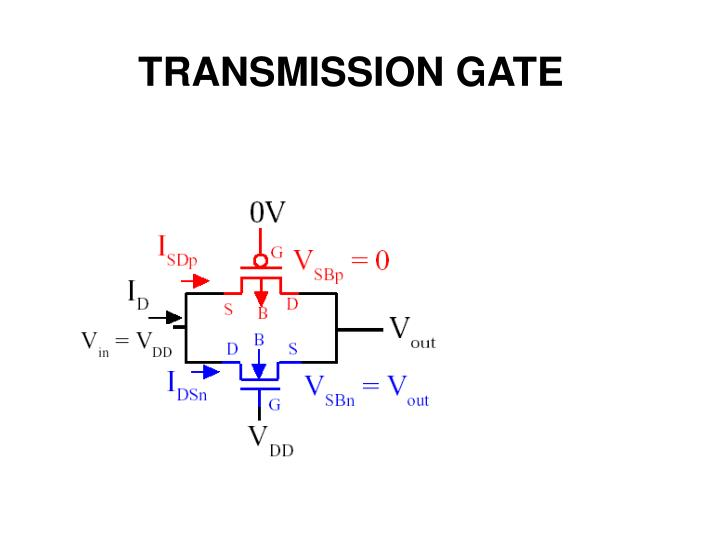
\includegraphics[width=8cm]{transmission-gate-n}
        \caption{\label{fig:transmission-gate-n}NMOS开关输出信号}
    \end{figure}
    \par 在传输门接法下,开关的导通电阻为:
    \begin{align}
        R_{on} = \frac{1}{\mu_nC_{ox}(\frac{W}{L})_n(VDD-V_{TN}) - \mu_pC_{ox}(\frac{W}{L})_p|V_{TP}| + [\mu_pC_{ox}(\frac{W}{L})_p-\mu_nC_{ox}(\frac{W}{L})_n]V_{in} }
    \end{align}
    \par 因此,当
    \begin{align}
        \mu_pC_{ox}(\frac{W}{L})_p=\mu_nC_{ox}(\frac{W}{L})_n] 
    \end{align}
    开关导通电阻与输入电压无关。
    \par 利用HSPICE仿真,可以得到传输门开关的大致性能。
    如\autoref{fig:tg}和\autoref{fig:tg_d},可以发现其相对与NMOS开关有
    明显的性能提升,不失为S/H电路与MDAC电路中开关的选择。
    \begin{figure}[H]
        \centering
        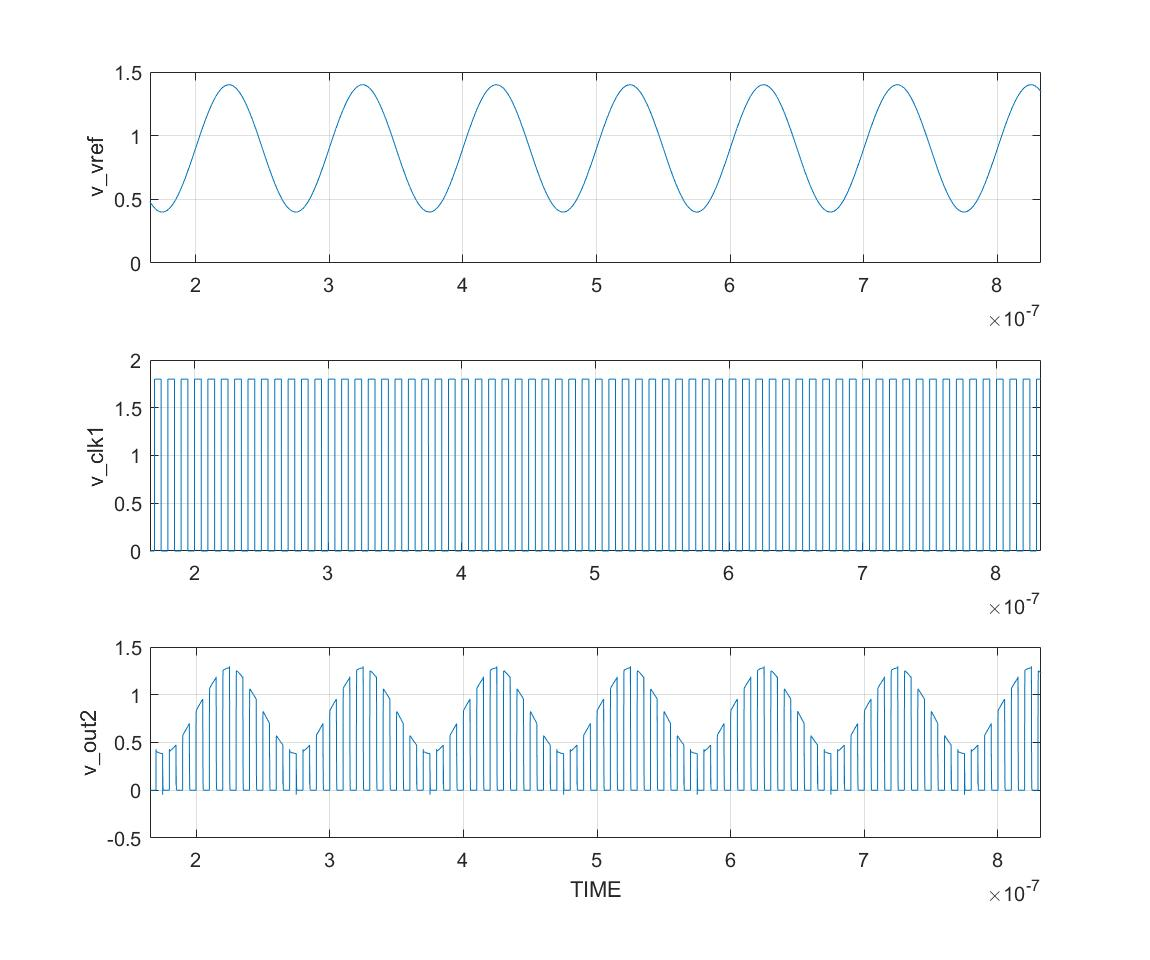
\includegraphics[width=8cm]{transgate}
        \caption{\label{fig:tg}传输门开关电路仿真}
    \end{figure}
    \begin{figure}[H]
        \centering
        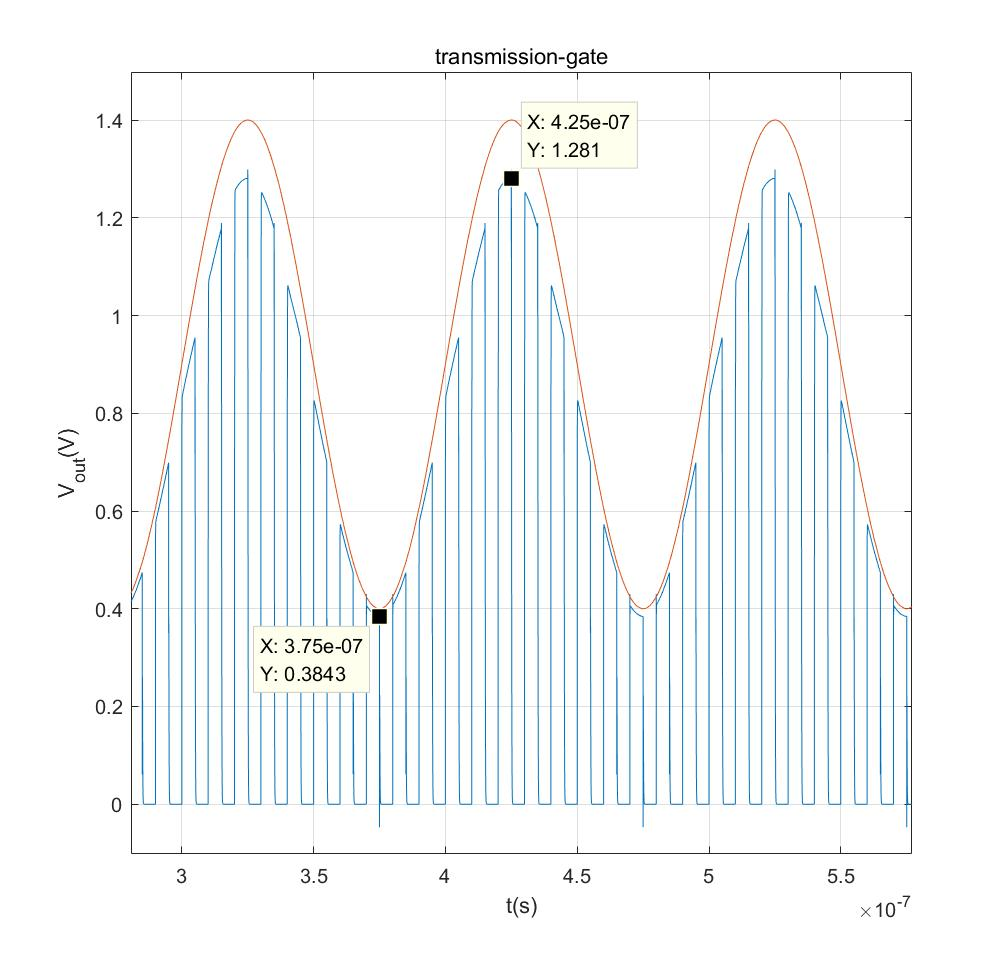
\includegraphics[width=8cm]{tg_d}
        \caption{\label{fig:tg_d}传输门开关输出信号}
    \end{figure}
    
    \par 传输门开关电路的cdl文件,如\autoref{code:TRANSGATE}所示。
    计算机学院的代码样式可能与其他专业不同,
    如有需要,可以从计算机学院专业模板中复制相关的代码样式设定。

    \begin{lstlisting}[%
        language={C},
        caption={TRANSGATE.cdl},
        label={code:TRANSGATE}
    ]
    ********************************************************************************
    * Library Name: Pipeline_ADC
    * Cell Name: transgate
    * View Name: schematic
    ********************************************************************************
    
    .SUBCKT transgate vdd gnd vin out clk
    XI0 clk clkb gnd vdd / inv_dac
    M1 vin clk out gnd n18 W=20u L=200n m=1
    M2 vin clkb out vdd p18 W=40u L=200n m=1
    
    .ENDS
    \end{lstlisting}

    \subsubsection{栅压自举式开关(bootstrap)}
    栅压自举式开关是一种应用在高速低功耗电路中的开关,其优势在于能够在不增加电路
    复杂度的情况下,提高速度和线性度。利用栅压自举技术,能够改善信号传输过程中的
    衰减与失真,避免导通电阻变化的问题。其电路如\autoref{fig:boot}所示。
    \begin{figure}[ht]
        \centering
        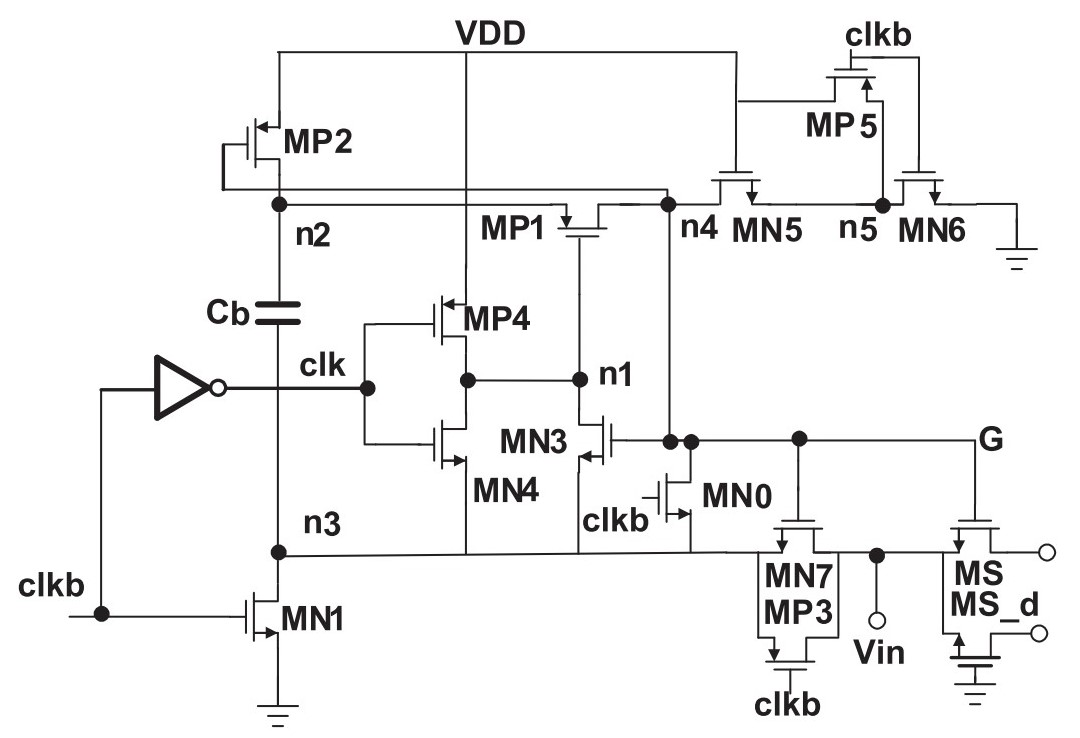
\includegraphics[width=8cm]{boot}
        \caption{\label{fig:boot}栅压自举式开关电路}
    \end{figure}
    \par MS是开关输出管,$ C_b $是为MS充电的电容。为减小MS处于“开”状态时的寄生电容,
    加入了MP5,同时也提高了系统的线性度。MN0与MP3能够提高开关的翻转速度。
    \par 当处于“关”状态时,clk为低电平,clkb为高电平,MN1导通,$ C_b $下极板接地。
    MN5和MN6导通,节点n4为低电平,则MP2导通,此时$ C_b $上极板接VDD,电容充电。
    MN7断开,MP4导通,n1节点为高电平,所以MP1断开,从而将MS与$ C_b $断开,此时MS断开,
    开关输出为0。MP5导通,MN5断开,D极电压减小,从而降低了节点n4的寄生电容。
    \par 当处于“开”状态时,clk为高电平,clkb为低电平,MN4导通MP1的G极接低电压,而S
    极接高电压,MP1导通。节点n4为高电平,所以MN7和MS导通。由于MS工作在线性区,
    其导通电阻较小,系统拥有较宽的通带。
    \par 利用HSPICE仿真,可以得到栅压自举式开关的大致性能。
    如\autoref{fig:bootstrap}和\autoref{fig:bootstrap_d},整体性能较好,毛刺较少,
    可以运用在关键的采样电路。
    \begin{figure}[H]
        \centering
        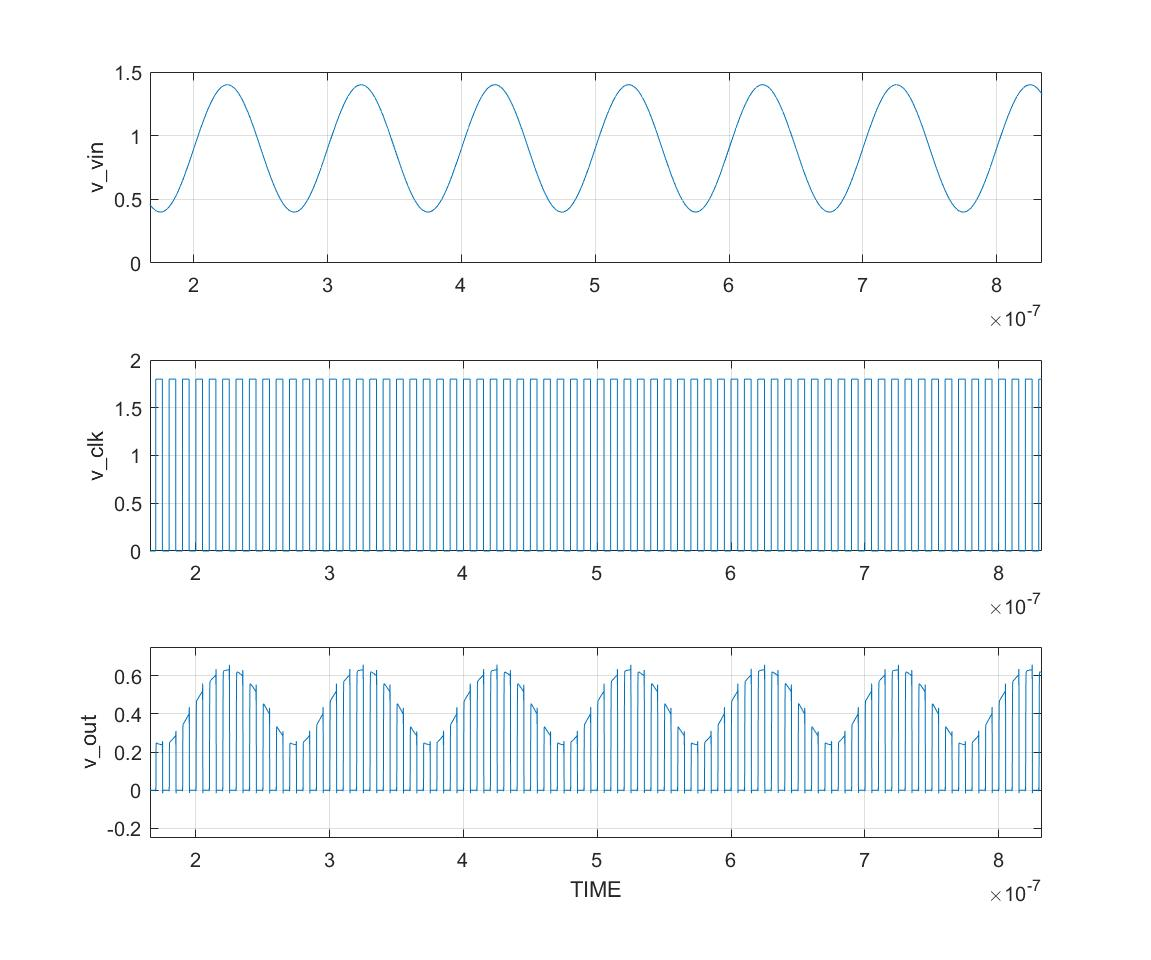
\includegraphics[width=8cm]{bootstrap}
        \caption{\label{fig:bootstrap}栅压自举式开关电路仿真}
    \end{figure}
    \begin{figure}[H]
        \centering
        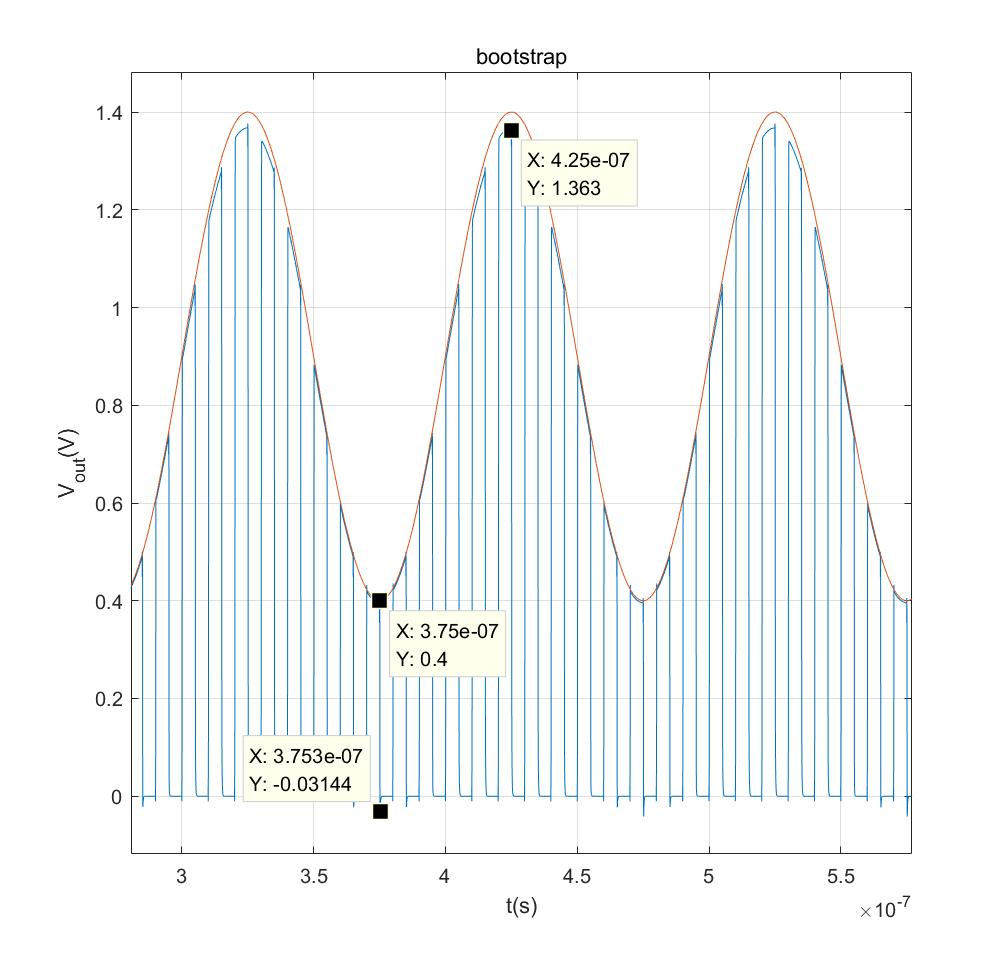
\includegraphics[width=8cm]{bootstrap_d}
        \caption{\label{fig:bootstrap_d}栅压自举式开关输出信号}
    \end{figure}
    \par 为进一步测试栅压自举式开关性能,利用MATLAB画图功能对其压摆率进行测试,如\autoref{fig:bootstrap_SR}所示。
    \begin{align}
        SR = \frac{1.152V-0.1372V}{0.0002\mu s} = 5074V/\mu s
    \end{align}
    \begin{figure}[ht]
        \centering
        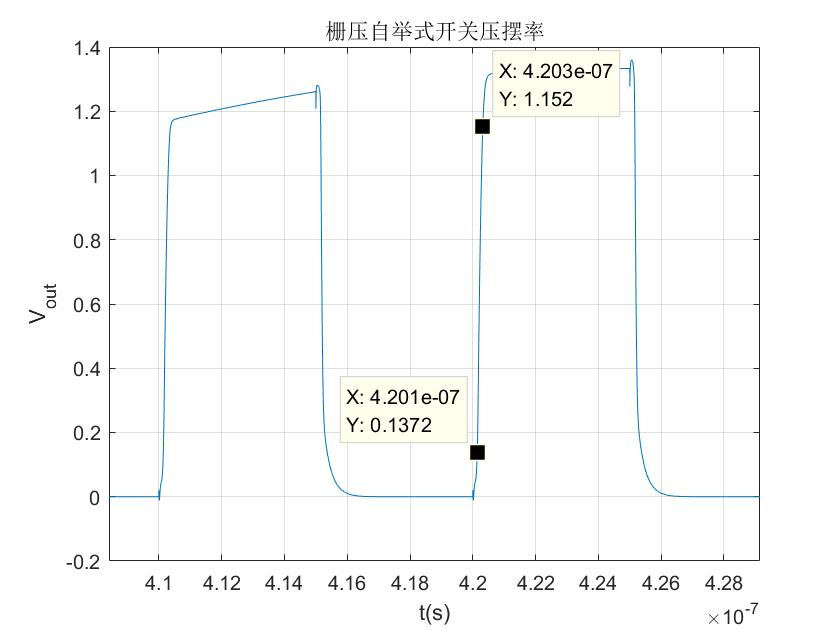
\includegraphics[width=8cm]{bootstrap_SR}
        \caption{\label{fig:bootstrap_SR}栅压自举式开关压摆率}
    \end{figure}
    \par 可见,栅压自举式开关压摆率较高,电路响应速率较快,能够在较高速的要求下工作。

    \par 栅压自举式开关电路的cdl文件,如\autoref{code:BOOTSTRAP}所示。
    计算机学院的代码样式可能与其他专业不同,
    如有需要,可以从计算机学院专业模板中复制相关的代码样式设定。

    \begin{lstlisting}[%
        language={C},
        caption={BOOTSTRAP.cdl},
        label={code:BOOTSTRAP}
    ]
    ********************************************************************************
    * Library Name: Pipeline_ADC
    * Cell Name: bootstrap
    * View Name: schematic
    ********************************************************************************

    .SUBCKT bootstrap vdd gnd vin out clk
    XI0 clk clkb gnd vdd / inv_dac
    MN1 n3 clkb gnd gnd n18 W=20u L=200n m=1
    MP2 n2 n4 vdd vdd p18 W=20u L=200n m=1
    MP4 n1 clk vdd vdd p18 W=20u L=200n m=1
    MN4 n1 clk n3 gnd n18 W=20u L=200n m=1
    MP1 n4 n1 n2 vdd p18 W=20u L=200n m=1
    MN3 n1 n4 n3 gnd n18 W=20u L=200n m=1
    MN5 n4 vdd n5 gnd n18 W=20u L=200n m=1
    MN7 vin n4 n3 gnd n18 W=20u L=200n m=1
    MP3 vin clkb n3 vdd p18 W=20u L=200n m=1
    MP5 vdd clkb n5 vdd p18 W=20u L=200n m=1
    MN6 n5 clkb gnd gnd n18 W=20u L=200n m=1
    MNS out n4 vin gnd n18 W=20u L=200n m=1

    Cb n2 n3 200f

    .ENDS
    \end{lstlisting}


\subsection{比较器}
比较器通过比较输入电压$ V_{in} $与参考电压$ V_{ref} $的大小,输出1或0的
数字码:若$ V_{in} > V_{ref} $输出高电平;若$ V_{in} < V_{ref} $输出
低电平。
    \subsubsection{静态比较器}
    \par 一种简单的思路,是利用运放的放大特性,如\autoref{fig:com}。由于理想运放开环增益$ A_v -> \infty $,
    因此当$ V_{in} $比$ V_{ref} $略大时,运放就能够把差分输入放大到饱和(VDD);同样,
    当$ V_{in} $比$ V_{ref} $略小时,运放就能够把差分输入放大到负的饱和(VSS)。
    \begin{figure}[H]
        \centering
        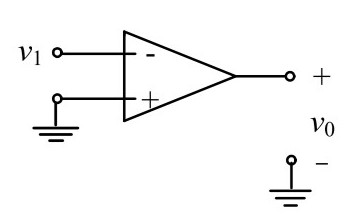
\includegraphics[width=8cm]{com}
        \caption{\label{fig:com}单门限电压比较器}
    \end{figure}
    \par 尽管电路非常简单,但这种比较器带来了两方面问题。
    \par 一是误差较大、精度较低。如\autoref{fig:com_os},可以看出,单门限电压比较器
    存在失调电压
    \begin{align}
        V_{os} \approx 0.3V
    \end{align}
    \begin{figure}[H]
        \centering
        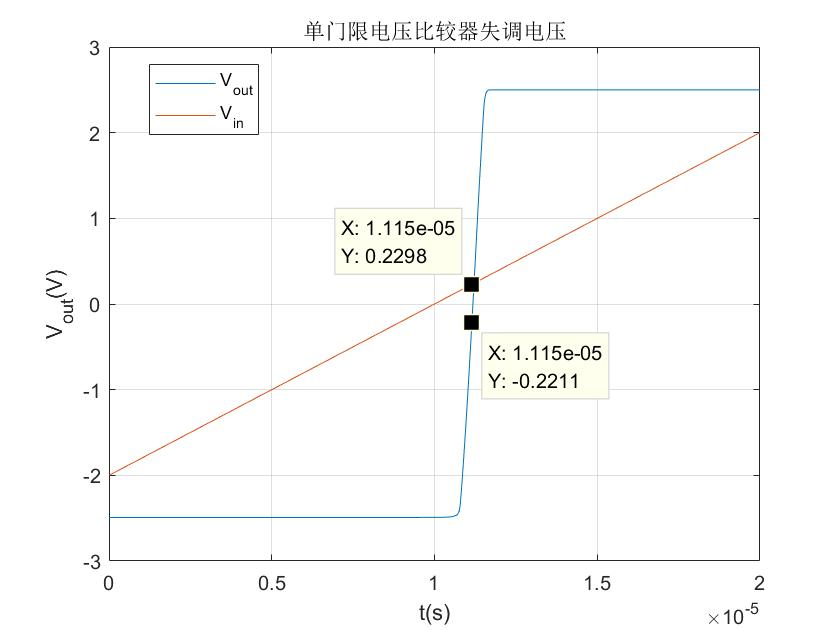
\includegraphics[width=10cm]{com_os}
        \caption{\label{fig:com_os}单门限电压比较器失调电压}
    \end{figure}

    \par 如\autoref{fig:com_result}同时可以计算得到其压摆率
    \begin{align}
        SR = \frac{2.499V-(-0.393V)}{0.56\mu s} = 5.16V/\mu s
    \end{align}
    \begin{figure}[H]
        \centering
        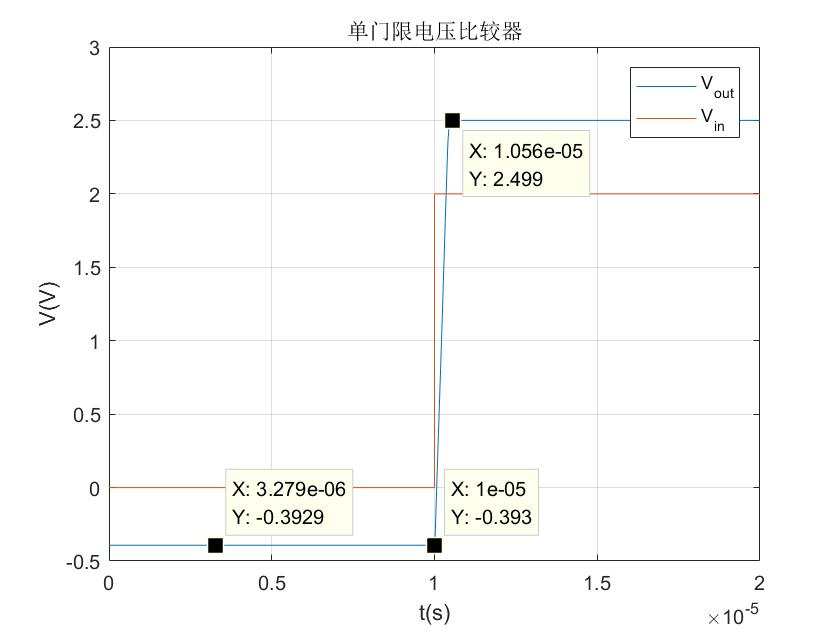
\includegraphics[width=10cm]{com_result}
        \caption{\label{fig:com_result}单门限电压比较器压摆率}
    \end{figure}

    \par 二是静态比较器的功耗较大,由于运放本身消耗功率较大,同时比较器一直处于
    工作状态,与流水线ADC低功耗的要求相悖。
    \subsubsection{动态比较器}
    动态比较器是为了解决静态比较器功耗大而提出的模型,其利用时钟信号clk来控制
    比较器是否运行,从而将比较器静态功率减为0,仅在工作时段存在功耗。常用
    的基本动态比较器主要有电阻分配式比较器、差分对比较器和电荷分配型比较器,
    他们的主要参数如\autoref{tab:com}:
    \begin{table}[ht]
        \caption{\label{tab:com}几种动态比较器参数对比}
        \begin{tabularx}{\linewidth}{|c|X<{\centering}|c|X<{\centering}|c|X<{\centering}|}
            \hline
            种类 & 失调电压 & 回踢噪声 & 比较速度 & 面积 & 功耗\\ \hline
            电阻分配式 & 大 & 小 & 慢 & 小 & 小\\ \hline
            差分对型 & 小 & 大 & 快 & 中 & 中\\ \hline
            电荷分配型 & 小 & 中 & 中 & 大 & 大\\ \hline
        \end{tabularx}
    \end{table}
    \par 考虑到系统高速低功耗的要求,论文采用如\autoref{fig:comparator}所示的动态比较器。
    \begin{figure}[H]
        \centering
        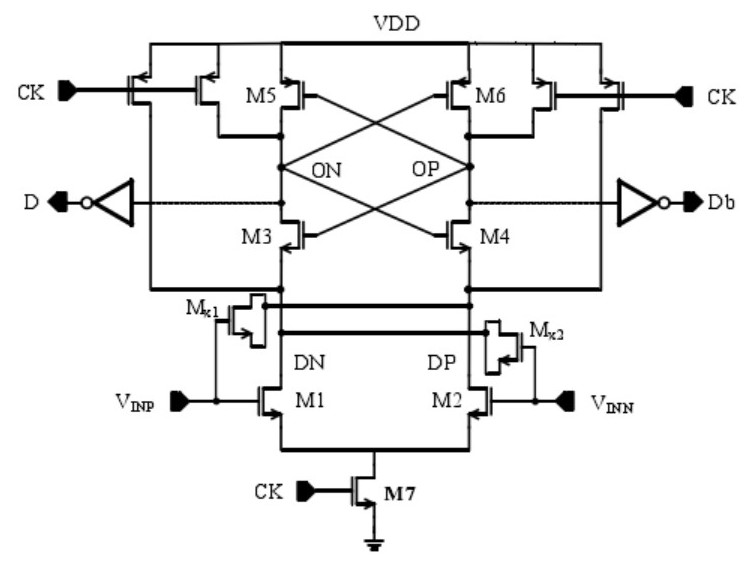
\includegraphics[width=8cm]{comparator}
        \caption{\label{fig:comparator}动态比较器电路}
    \end{figure}
    \par 当clk为低电平时,比较器在复位阶段,M1和M2的D极,节点ON与OP经M5与M6两侧的PMOS管接到VDD。
    当clk为高电平时,M7导通,节点DN与DP电压下降,由于M1与M2的G极电压不同($ V_{ip} < V_{in} $),
    两节点电压下降速度不同(DP更快),当$ V_{DP} < VDD - V_{TN} $时,M6导通,M4导通,从而节点OP电压
    下降,节点ON电压上升,经过反相器后,输出高电平。最终实现对$ V_{in} $与$ V_{ip} $的比较。反相器
    用于增强输出的驱动能力,同时能够有效减少输出毛刺。
    \par 利用HSPICE仿真,可以得到动态比较器的大致性能,如\autoref{fig:comparator_perform}。
    \begin{figure}[H]
        \centering
        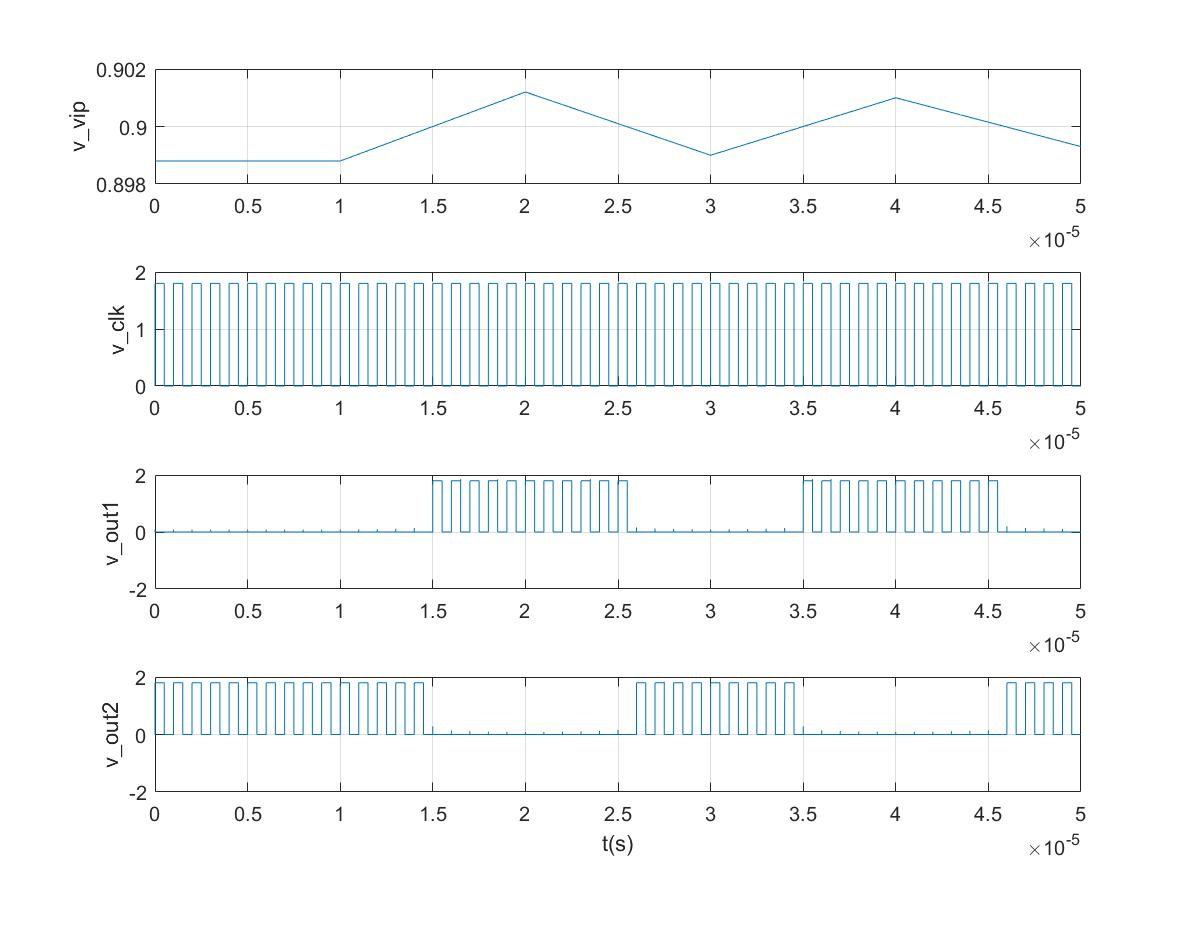
\includegraphics[width=10cm]{comparator_perform}
        \caption{\label{fig:comparator_perform}动态比较器仿真}
    \end{figure}
    \par 通过设置合适的输入电压,能够得到比较器的失调电压和压摆率,如\autoref{fig:comparator_os}和\autoref{fig:comparator_SR}
    \begin{figure}[H]
        \centering
        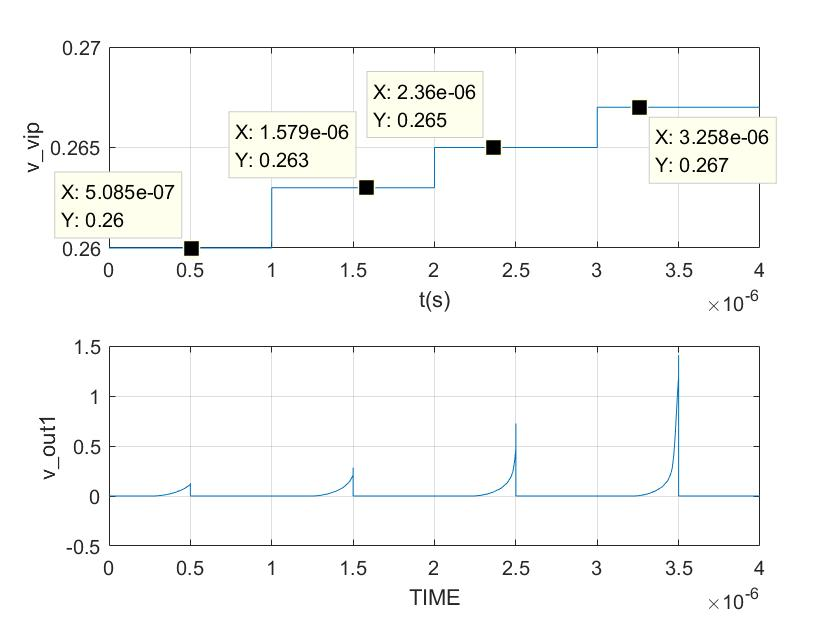
\includegraphics[width=10cm]{comparator_os}
        \caption{\label{fig:comparator_os}动态比较器失调电压}
    \end{figure}
    \par 可以看出,当$ V_{in} = 0.267V $时,输出电压基本可视作毛刺。
    因此,可以取
    \begin{align}
        V_{os} \approx 0.27V
    \end{align}
    \begin{figure}[H]
        \centering
        \includegraphics[width=10cm]{comparator_SR}
        \caption{\label{fig:comparator_SR}动态比较器压摆率}
    \end{figure}
    \par 由于变化的时间过小,在图中无法得出准确的数值,经过查询HPSICE仿真得到的.lis文件
    可以大致计算压摆率
    \begin{align}
        SR = \frac{1.6043V-0.1526V}{5.0002645\mu s-5.000236\mu s} = 5.09\times10^{4}V/\mu s
    \end{align}
    \par 可见,其压摆率极高,精确度高,响应速率快,能够满足电路高速的要求。
    \par 由于在仿真过程中,宽长比均取为$ \frac{20}{0.2} $并非该电路的最佳参数,所以失调电压
    相对静态比较器并没有相当大的提升。不过,其理想状态下,失调电压可以控制在5.62mV,在冗余位校正
    技术的容许范围之内。
    \par 注意到,这里使用的动态比较器仅在时钟为高电平的时候工作,在时钟低电平的时候不工作,这一方面
    带来了降低功耗的优势;另一方面,给后续的sub-ADC电路和MDAC电路的设计带来一定的难度,由于输入信号
    均只有固定的有效时间,都需要时钟信号来控制工作。为实现后续电路的时钟逻辑,应加入寄存器等电路,
    由于这部分内容更贴近与数字电路,论文不再进一步深究。

    \par 比较器电路的cdl文件,如\autoref{code:COMPARATOR}所示。
    计算机学院的代码样式可能与其他专业不同,
    如有需要,可以从计算机学院专业模板中复制相关的代码样式设定。

    \begin{lstlisting}[%
        language={C},
        caption={COMPARATOR.cdl},
        label={code:COMPARATOR}
    ]
    ********************************************************************************
    * Library Name: Pipeline_ADC
    * Cell Name: comparator
    * View Name: schematic
    ********************************************************************************

    .SUBCKT comparator vdd gnd vip vin outp clk

    XI0 n3 outp gnd vdd / inv_dac
    XI1 n4 outn gnd vdd / inv_dac
    MN1 n1 vip n5 gnd n18 W=20u L=0.2u m=1
    MN2 n2 vin n5 gnd n18 W=20u L=0.2u m=1
    MN3 n3 n4 n1 gnd n18 W=20u L=0.2u m=1
    MN4 n4 n3 n2 gnd n18 W=20u L=0.2u m=1
    MP1 n1 clk vdd vdd p18 W=20u L=0.2u m=1
    MP2 n3 clk vdd vdd p18 W=20u L=0.2u m=1
    MP3 n3 n4 vdd vdd p18 W=20u L=0.2u m=1
    MP4 n4 n3 vdd vdd p18 W=20u L=0.2u m=1
    MP5 n4 clk vdd vdd p18 W=20u L=0.2u m=1
    MP6 n2 clk vdd vdd p18 W=20u L=0.2u m=1
    MNX1 n2 vip n2 gnd n18 W=20u L=0.2u m=1
    MNX2 n1 vin n1 gnd n18 W=20u L=0.2u m=1
    MN7 n5 clk gnd gnd n18 W=20u L=0.2u m=1

    .ENDS
    \end{lstlisting}


\subsection{sub-ADC电路}
    \subsubsection{sub-ADC电路仿真}
    sub-ADC采用全平行结构ADC,论文采用的第一级子结构为2.5bitMDAC,因此对应的sub-ADC需要6个比较器
    对应的参考电压为:
    \begin{align*}
        V_{ref1} & = -0.625 \\
        V_{ref2} & = -0.375 \\
        V_{ref3} & = -0.125 \\
        V_{ref4} & = 0.125 \\
        V_{ref5} & = 0.375 \\
        V_{ref6} & = 0.625 \\
    \end{align*}
    \par 将6个比较器的一个输入端接输入信号,另一个输入端接对应参考电压。由于论文仅涉及流水线ADC的子结构部分,
    而未对后续的数字校正电路实现,因此,此处sub-ADC的输出仅为6个比较器的输出,而非对应的数字码。同时,
    直接输出六个比较器的比较结果,简化了对子结构中DAC的要求,利用简单的信号处理,便能得到该级的放大余量,详细
    内容在4.5小节叙述。
    \par 利用HSPICE仿真,可以得到sub-ADC的输出波形,如\autoref{fig:subADC_out}。
    \begin{figure}[H]
        \centering
        \includegraphics[width=12cm]{subADC_out}
        \caption{\label{fig:subADC_out}sub-ADC的六个输出}
    \end{figure}
    \par 当$ V_{in} > V_{refi} $时,第i个比较器在工作时间内输出高电平,可以看出sub-ADC处于正常工作状态。

    \subsubsection{参考电压的产生}
    一种简单的思路是直接利用对应的电压源作为参考电压,但是考虑到电路整体功耗,
    这种方式不可取。
    \par 另一种思路是利用电阻对供电电压分压,得到对应的参考电压。这种方法
    需要电阻阻值成一定比例(11:2:2:2:2:2:11),如\autoref{fig:v_ref}。
    \begin{figure}[H]
        \centering
        \includegraphics[width=2cm]{v_ref}
        \caption{\label{fig:v_ref}参考电压的产生}
    \end{figure}
    \par 利用该分压电路进行仿真后,发现sub-ADC输出出现问题,所有比较器均提前输出高电平,
    如\autoref{fig:subADC_error}。
    \begin{figure}[H]
        \centering
        \includegraphics[width=12cm]{subADC_error}
        \caption{\label{fig:subADC_error}sub-ADC错误输出}
    \end{figure}
    \par 细究其原因,是比较器电路中的电容、MOS管,影响了参考电压电路的稳定性,
    使其在工作过程中,出现了较明显的毛刺,最终导致比较器误判而提前输出高电平。
    如\autoref{fig:error}。
    \begin{figure}[H]
        \centering
        \includegraphics[width=12cm]{error}
        \caption{\label{fig:error}参考电压毛刺导致比较器错误}
    \end{figure}
    \par 参考电压的毛刺摆幅将近3V,为得到稳定的参考电压,一种方法是在参考电压输出端
    接电压跟随器,从而隔绝前后电路阻抗的相互影响,如\autoref{fig:v_ref_fol}。
    \begin{figure}[H]
        \centering
        \includegraphics[width=4cm]{v_ref_fol}
        \caption{\label{fig:v_ref_fol}参考电压的产生}
    \end{figure}
    \par 直接加入6个运放,对电路功耗是一个巨大的压力,为达到低功耗的特性,利用电容
    滤波,无疑是一种更优的解决方案。如\autoref{fig:v_ref_c}。
    \begin{figure}[H]
        \centering
        \includegraphics[width=3cm]{v_ref_c}
        \caption{\label{fig:v_ref_c}参考电压的产生}
    \end{figure}
    \par 使用改进后的参考电压电路,比较器的工作状态恢复正常,
    如\autoref{fig:fix_error}。
    \begin{figure}[H]
        \centering
        \includegraphics[width=12cm]{fix_error}
        \caption{\label{fig:fix_error}参考电压滤波后比较器输出}
    \end{figure}

    \par sub-ADC电路的cdl文件,如\autoref{code:sub-ADC}所示。
    计算机学院的代码样式可能与其他专业不同,
    如有需要,可以从计算机学院专业模板中复制相关的代码样式设定。

    \begin{lstlisting}[%
        language={C},
        caption={SUBADC.cdl},
        label={code:sub-ADC}
    ]
    ********************************************************************************
    * Library Name: Pipeline_ADC
    * Cell Name: subadc
    * View Name: schematic
    ********************************************************************************

    .SUBCKT subadc vdd vss gnd vip out1 out2 out3 out4 out5 out6 clk

    //create reference voltage for flash adc
    R1 vss ref1 11k
    R2 ref1 ref2 2k
    R3 ref2 ref3 2k
    R4 ref3 ref4 2k
    R5 ref4 ref5 2k
    R6 ref5 ref6 2k
    R7 ref6 vdd 11k

    //use capacitors to eliminate flunctuation
    C1 ref1 gnd 1n
    C2 ref2 gnd 1n
    C3 ref3 gnd 1n
    C4 ref4 gnd 1n
    C5 ref5 gnd 1n
    C6 ref6 gnd 1n

    //compare the input with the reference voltage
    XC1 vdd vss vip ref1 out1 clk / comparator
    XC2 vdd vss vip ref2 out2 clk / comparator
    XC3 vdd vss vip ref3 out3 clk / comparator
    XC4 vdd vss vip ref4 out4 clk / comparator
    XC5 vdd vss vip ref5 out5 clk / comparator
    XC6 vdd vss vip ref6 out6 clk / comparator

    .ENDS
    \end{lstlisting}


\subsection{MDAC电路}
    MDAC电路的功能实质上是将输入电压与sub-ADC采样电压做差,并将余量重新
    放大到满量程,即$ V_{redisue} = k(V_{in} - V_{adc}) $。由于2.5bitMDAC
    的输入输出关系已确定:
    \begin{align}
        V_{\text {out}}=
        \left\{
        \begin{array}{ccc}
            4V_{in} + 3V & -1V \leq V_{in} < -0.625V \\
            4V_{in} + 2V & -0.625V \leq V_{in} < -0.375V \\
            4V_{in} + 1V & -0.375V \leq V_{in} < -0.125V \\
            4V_{in} & -0.125V \leq V_{in} < 0.125V \\
            4V_{in} - 1V & 0.125V \leq V_{in} < 0.375V \\
            4V_{in} - 2V & 0.375V \leq V_{in} < 0.625V \\
            4V_{in} - 3V & 0.625V \leq V_{in} < 1V \\
       \end{array}
        \right.
    \end{align}
    \par 利用电压加法电路,直接将各比较器输出电压缩放后相加,得到从0-6V的叠加信号,
    减去3V固定电平,使得输出信号在$[-3V,\ 3V]$范围内。在利用减法电路与放大的输入信号做差,
    就能够实现余量放大功能,如\autoref{fig:MDAC_sim}。
    \begin{figure}[ht]
        \centering
        \includegraphics[width=10cm]{MDAC_sim}
        \caption{\label{fig:MDAC_sim}MDAC电路结构图}
    \end{figure}
    \par 在实际仿真过程中,由于4.1节中的运算放大器存在非理想性,构建加法电路
    的过程中存在一定的误差,当6路信号的误差累加后最终输出偏差较大。因此,在HSPICE仿真
    过程中采取的策略是:利用一个7路加法电路,一个反相放大器,一个反相器。加法电路将各比较器
    输出以$ \frac{1}{10} $比例相加,输入信号经反相器后放大1.6倍接入加法电路,最后将加法电路
    输出反相放大1.5倍,可以得到较为理想的输出。如\autoref{fig:MDAC_clk_ref}。
    \begin{figure}[H]
        \centering
        \includegraphics[width=10cm]{MDAC_clk_ref}
        \caption{\label{fig:MDAC_clk_ref}MDAC电路输出}
    \end{figure}

    \par MDAC电路的cdl文件,如\autoref{code:MDAC}所示。
    计算机学院的代码样式可能与其他专业不同,
    如有需要,可以从计算机学院专业模板中复制相关的代码样式设定。

    \begin{lstlisting}[%
        language={C},
        caption={MDAC.cdl},
        label={code:MDAC}
    ]
    ********************************************************************************
    * Library Name: Pipeline_ADC
    * Cell Name: madc
    * View Name: schematic
    ********************************************************************************

    .SUBCKT mdac vdd vss gnd in1 in2 in3 in4 in5 in6 in7 out

    //invert the input
    XI0 vdd vss in7 in7n / invertor

    //add 7 signal
    XI1 gnd in outt vdd vss / OPAMP
    R0 in outt 100k
    Ra in1 in 1000k
    Rb in2 in 1000k
    Rc in3 in 1000k
    Rd in4 in 1000k
    Re in5 in 1000k
    Rf in6 in 1000k
    Ri in7n in 62k

    //residue amplify
    XI2 outt vin2 out vdd vss / OPAMP
    R2f out vin2 150k
    R21 vin2 gnd 100k

    .ENDS
    \end{lstlisting}



\subsection{第一级子电路总体仿真}
    \subsubsection{总体电路参数}
    根据HSPICE仿真,第一级子电路总体参数如\autoref{tab:para}
    \begin{table}[ht]
        \centering
        \caption{\label{tab:para}第一级子电路参数}
        \begin{tabular}{|c|c|}
            \hline
            工作电压 & $ \pm 2V $ \\ \hline
            最大工作速率 & $1MSPS$ \\ \hline
            比特数 & $2.5$  \\ \hline
            功耗 & $134.8mW$  \\ \hline
        \end{tabular}
    \end{table}
    \par 第一级子电路HSPICE仿真代码,如\autoref{code:sub}所示。
    计算机学院的代码样式可能与其他专业不同,
    如有需要,可以从计算机学院专业模板中复制相关的代码样式设定。

    \begin{lstlisting}[%
        language={C},
        caption={sub.sp},
        label={code:sub}
    ]
    .title firststage

    .include 'OPA.cdl'
    .include 'INVERTOR.cdl'
    .include 'SUBADC.cdl'
    .include 'COMPARATOR.cdl'
    .include 'INV.cdl'
    .include 'MDAC.cdl'

    VVDD vdd 0 DC = 2V
    VGND gnd 0 0
    VVSS 0 vss DC = 2V
    VVip vip 0 pwl 0 -1, 1m 1
    VCLK clk 0 pulse(0 1.8 0 1p 1p 5u 10u)

    //sub-ADC电路
    XA0 vdd vss gnd vip out1 out2 out3 out4 out5 out6 clk / subadc

    //MDAC电路
    XM0 vdd vss gnd out1 out2 out3 out4 out5 out6 vip out / mdac

    //瞬态仿真
    .tran 1n 1m
    .probe v(vip) v(out)
    //计算功耗
    .measure powerall avg power

    .lib '..\models\ms018.lib' tt
    .temp 27
    .option post accurate probe nomod captab
    .end
    \end{lstlisting}


    \subsubsection{电路总体速率}
    论文提出的子结构理论上工作速率应当满足1GSPS的要求,其中,传输门开关、栅压自举式开关和比较器
    电路均能工作在较高速率,然而,4.1节中设计的运算放大器极大地限制了整体电路的工作速率。
    \begin{table}[ht]
        \centering
        \caption{\label{tab:SR_com}子结构中各模块压摆率对比}
        \begin{tabular}{|c|c|c|}
            \hline
            模块 & $SR(V/\mu s)$ \\ \hline
            栅压自举式开关 & $5074$ \\ \hline
            动态比较器 & $5.09\times 10^4$ \\ \hline
            运算放大器 & $10.72$ \\ \hline
            sub-ADC & $5.09\times 10^4$ \\ \hline
            MDAC & $10.72$ \\ \hline
        \end{tabular}
    \end{table}
    \par 如\autoref{tab:SR_com},子结构的工作速率不能太高,否则,由于运算放大器响应速率低,
    将导致MDAC中的加法电路无法正常工作,从而导致子结构整体输出错误。
    \par 如果将电路的时钟频率增加,则能够明显地看出电路响应速率的问题。
    \par 如\autoref{fig:MDAC_clk_ref},4.5节中的MDAC工作速率为0.1MSPS,输出波形正常。
    \begin{figure}[H]
        \centering
        \includegraphics[width=8cm]{MDAC_clk_ref}
        \caption{\label{fig:MDAC_clk_ref}MDAC电路输出(0.1MSPS)}
    \end{figure}
    \par 如\autoref{fig:1M_whole},若将工作速率增加为1MSPS,输出波形大体正常,
    但能够看出每个时钟内信号无法很好地保持,如\autoref{fig:1M}。
    \begin{figure}[H]
        \centering
        \includegraphics[width=8cm]{1M_whole}
        \caption{\label{fig:1M_whole}MDAC电路输出(1MSPS)}
    \end{figure}
    \begin{figure}[H]
        \centering
        \includegraphics[width=8cm]{1M}
        \caption{\label{fig:1M}MDAC电路输出细节(1MSPS)}
    \end{figure}
    \par 如\autoref{fig:10M_whole},若将工作速率继续增加为10MSPS,输出波形已经完全错误,
    MDAC中的加法器已经无法正常工作。
    \begin{figure}[H]
        \centering
        \includegraphics[width=8cm]{10M_whole}
        \caption{\label{fig:10M_whole}MDAC电路输出(10MSPS)}
    \end{figure}

    \subsubsection{电路总体功耗}
    对比TI公司的几款高速ADC,一般达到1GSPS的高速低功耗ADC性能参数如\autoref{tab:speed_com}
    \begin{table}[ht]
        \centering
        \caption{\label{tab:speed_com}TI公司流水线ADC功耗}
        \begin{tabular}{|c|c|c|c|c|}
            \hline
            型号 & 速率(GSPS) & 比特数 & 通道数 & 功耗(W) \\ \hline
            AFE7422 & $3$ & $ 14 $ & $2$ & $ 8.2 $ \\ \hline
            ADC31RF80 & $3$ & $ 14 $ & $1$ & $ 3.2 $ \\ \hline
            ADS54J64 & $0.5-1$ & $ 14 $ & $4$ & $ 2.5 $ \\ \hline
        \end{tabular}
    \end{table}
    \par 利用HSPICE仿真,可以得到第一级子电路在1MSPS工作速率下
    的总体功耗,如\autoref{fig:all_power}
    \begin{align}
        P_{sub} = 134.8mW
    \end{align}
    \begin{figure}[H]
        \centering
        \includegraphics[width=8cm]{all_power}
        \caption{\label{fig:all_power}第一级子电路功率出(10MSPS)}
    \end{figure}
    \par 根据此第一级子电路估计,完整的流水线ADC电路功率约5个子结构加上数字
    校正电路的功耗之和,保守估计大约$ 1W $,由于电路无法工作以大于10MSPS的速率
    工作,因此无法得知约1GSPS速率下功耗。
    \begin{align}
        P_{whole} \geq 5P_{sub} + P_{rect} \approx 1W
    \end{align}

\section{总结与感想}
    \subsection{工作总结}
    本次电子电路基础专题研究报告以高速低功耗的12bit1GSPS的SHA-less型流水线ADC为出发点,先重新
    梳理了流水线ADC的工作原理,分别探究了SHA-less架构和动态比较器两种
    低功耗技术,利用Simulink进行了行为级仿真,验证了在非理想状态下,SHA-less
    架构的流水线ADC相比传统流水线ADC拥有更低的功耗和噪声;同时利用HSPICE设计
    了一款满足一定要求的运算放大器以及流水线ADC中涉及的几个模块,
    对流水线ADC中第一级子电路进行了设计以及仿真。但是,受限于时间及能力,一方面设计
    的运算放大器远远无法达到高速工作的要求,在仿真过程中只能以1MSPS的速率测试;另一方面,
    对于完整的流水线ADC及其数字校正电路等均为完成,无法测试完整电路性能,只能进行粗略地估计,
    大致能够满足低功耗的要求;最后,由于采样保持电路的效果较差,加上利用时钟控制工作状态有
    一定的采样效果,因此在仿真中暂未加入各子电路中的S/H电路与MDAC电路中开关的选择。
    
    \subsection{课程感想}
    从去年12月开始至今,所有工作从书本第六章的仔细阅读,6.23运算放大器的设计与仿真,
    到12月中旬的SHA-less架构流水线ADC设计的主题确定,广泛地参考文献、书籍,一直到年底
    开始仿真与实现,最终撰写论文,整个过程十分漫长也非常煎熬,不过收获也很多。这是第一次真真切切
    地体会到了学术论文应该如何撰写的完整过程,还加强了\text{\LaTeX}的使用。虽然最终的成果不算非常成功,
    但至少Simulink的使用方法,HSPICE电路级的仿真,还有对流水线ADC当前技术的认识,都算受益匪浅。
    \par 关于电子电路基础课程,首先我感觉教的内容似乎有些少。尤其是前期花费过多时间在第一、第二章
    的基础内容,由于这两部分内容其实在信电导论课程中已经学习过,新的部分仅为系统函数和波特图,我觉得
    可以在前面部分加快课程进度,为后面内容以及更多拓展内容腾出时间。其次,我认为课程讲解部分不应该仅有
    课本上的内容,系统级工作中可以引入更多当前的新技术。如第六章的流水线ADC,书本上仅介绍了单通道
    的流水线ADC,然而实际上运用中,多通道的ADC更为常见,在多通道的基础上,又有时间交织技术、通道间
    运放共享技术,都是当前流水线ADC中研究的热点。而且在实际的运用中,集成电路不可或缺的拥有时钟信号,
    虽然这部分比较贴近数字电路课程,但如果书本上的电路均是连续工作而没有时钟控制的,在走出象牙塔真正接触
    集成电路的设计时就会面临巨大的鸿沟。
    \par 最后,我非常感谢电子电路基础这门课,给我带来了一个充实的秋冬学期。

